\documentclass[a4paper,12pt]{article}

\usepackage{amsthm}
\usepackage{amsmath}
\usepackage[framemethod=TikZ]{mdframed}
\usepackage{soul}
\usepackage{upgreek}
\usepackage{amssymb}
\usepackage{dsfont}
\usepackage{stmaryrd}
\usepackage{xcolor}
\usepackage[shortlabels]{enumitem}
\usepackage{hyperref}
\usepackage{pifont}
\usepackage{tikz}
\usepackage{verbatim}
\usepackage{graphicx}

\setlength\parindent{0pt}

% Definition
\newcounter{definition}[section]\setcounter{definition}{0}
\renewcommand{\thedefinition}{\arabic{section}.\arabic{definition}}
\newenvironment{definition}[2][]{%
\refstepcounter{definition}%
\ifstrempty{#1}%
{\mdfsetup{%
frametitle={%
\tikz[baseline=(current bounding box.east),outer sep=0pt]
\node[anchor=east,rectangle,fill=white]
{\strut Definition~\thedefinition};}}
}%
{\mdfsetup{%
frametitle={%
\tikz[baseline=(current bounding box.east),outer sep=0pt]
\node[anchor=east,rectangle,fill=white]
{\strut Definition~\thedefinition:~#1};}}%
}%
\mdfsetup{innertopmargin=3pt,linecolor=gray!50,%
linewidth=2pt,topline=true,%
frametitleaboveskip=\dimexpr-\ht\strutbox\relax
}
\begin{mdframed}[]\relax%
\label{#2}}{\end{mdframed}}
%%

% Theorem
\newcounter{theorem}[section]\setcounter{theorem}{0}
\renewcommand{\thetheorem}{\arabic{section}.\arabic{theorem}}
\newenvironment{theorem}[2][]{%
\refstepcounter{theorem}%
\ifstrempty{#1}%
{\mdfsetup{%
frametitle={%
\tikz[baseline=(current bounding box.east),outer sep=0pt]
\node[anchor=east,rectangle,fill=white]
{\strut Theorem~\thetheorem};}}
}%
{\mdfsetup{%
frametitle={%
\tikz[baseline=(current bounding box.east),outer sep=0pt]
\node[anchor=east,rectangle,fill=white]
{\strut Theorem~\thetheorem:~#1};}}%
}%
\mdfsetup{innertopmargin=3pt,linecolor=gray!50,%
linewidth=2pt,topline=true,%
frametitleaboveskip=\dimexpr-\ht\strutbox\relax
}
\begin{mdframed}[]\relax%
\label{#2}}{\end{mdframed}}
%%

% Lemma
\newcounter{lemma}[section]\setcounter{lemma}{0}
\renewcommand{\thelemma}{\arabic{section}.\arabic{lemma}}
\newenvironment{lemma}[2][]{%
\refstepcounter{lemma}%
\ifstrempty{#1}%
{\mdfsetup{%
frametitle={%
\tikz[baseline=(current bounding box.east),outer sep=0pt]
\node[anchor=east,rectangle,fill=white]
{\strut Lemma~\thelemma};}}
}%
{\mdfsetup{%
frametitle={%
\tikz[baseline=(current bounding box.east),outer sep=0pt]
\node[anchor=east,rectangle,fill=white]
{\strut Lemma~\thelemma:~#1};}}%
}%
\mdfsetup{innertopmargin=3pt,linecolor=gray!50,%
linewidth=2pt,topline=true,%
frametitleaboveskip=\dimexpr-\ht\strutbox\relax
}
\begin{mdframed}[]\relax%
\label{#2}}{\end{mdframed}}
%%

\newlist{todolist}{itemize}{2}
\setlist[todolist]{label=$\square$}

\newcommand{\cmark}{\ding{51}}%
\newcommand{\xmark}{\ding{55}}%
\newcommand{\done}{\rlap{$\square$}{\raisebox{2pt}{\large\hspace{1pt}\cmark}}%
\hspace{-2.5pt}}
\newcommand{\wontfix}{\rlap{$\square$}{\large\hspace{1pt}\xmark}}


\title{Master Thesis}
\date{\today}
\author{Sally Chau}

\begin{document}

\maketitle
\tableofcontents

\section{Preparation}

\subsection{Topic 1: Backward Confluence for Separation Logic/ Graph Grammars}

\subsubsection{Summary}
Both \ul{Graph Grammars} and \ul{Separation Logic} are used to represent Heap
Configurations.\\
Graph Grammars can be used to verify structural and relational properties
for heaps in shape analysis. For the state space generation (abstraction) to terminate, we have to check whether the program state of an abstracted heap configuration has already been encountered before. Otherwise a single loop in the program typically means that we will generate new states forever.
The question "has this abstract heap configuration been encountered before" is an instance of the \ul{language inclusion problem}:\\
We ask whether the language of a newly discovered abstract heap configuration
is included in the language of some previously discovered heap configuration, which is generally undecidable.\\
\ul{Backward confluence} is beneficial for abstraction, because instead of
applying all combinations of inverse derivation steps, we know that - no
matter in which combination we apply inverse derivations - we end up with the
same unique abstract heap configuration. Backward confluence does not exclude critical pairs of derivation rules. It rather requires that heap configurations arising from backward derivation steps using overlapping rules must be \ul{joinable}, i.e.,
(backwards) derivable to the same heap. Hence, backward confluence speeds up abstraction.\\
There are classes of Graph Grammars that can be constructed to be backward confluent, however, not all grammars obtain this property. \\
As a fragment of SL can be translated to Graph Grammars, results on
language inclusion and emptiness for Graph Grammars can be transferred to
entailment and satisfiability of SL. Thus, a possible result on backward
confluent Graph Grammars can also be transferred to SL.\\
Cyclic proofs are a semi-algorithm to decide the entailment (language inclusion problem) for SL. If we can find a cyclic proof, then we know that we found a solution. However, termination is not guaranteed.  

\subsubsection{Tasks}

\begin{enumerate}
	\item Define the subclass of graph grammars that can be constructed to be backward confluent.
	\item Transfer the notion of backward confluence to SL; properly formulate criteria, e.g. critical pairs, for SL to see whether these conditions are "natural" in an SL setting. How do the previous findings for graph grammars transfer to SL?
	\item Is it possible to design an algorithm to find cyclic proofs for backward confluent grammars/ predicates? What are the requirements?
\end{enumerate}

\subsubsection{Lecture on Static Program Analysis}

\paragraph{Lecture 1: Introduction to Program Analysis}

\begin{itemize}
	\item \ul{Static program analysis}: general method of automated reasoning of artefacts (requirements, design models, programs)
	\item Static: based on source code, not on dynamic execution
	\item Automated: little user intervention
	\item Applications
	\begin{itemize}
		\item Optimizing compilers: improve runtime, memory efficiency
		\item Software verification: verify program correctness
	\end{itemize}
	\item Correctness = Soundness + Completeness
\end{itemize}

\paragraph{Lecture 2: Dataflow Analysis I (Introduction and Available Expressions/ Live Variables Analysis)}

\begin{itemize}
	\item \ul{Dataflow Analysis}: describe how analysis information flows through program
	\begin{itemize}
		\item Dependence on statement order (flow-sensitive vs. flow-insensitive analyses)
		\item Direction of flow (forward vs. backward analyses)
		\item Quantification over paths (may (union) vs. must (intersection) analyses)
		\item Procedures (interprocedural vs intraprocedural analyses)
	\end{itemize}
	\item Define 
	\begin{itemize}
		\item labels to locate information incl. init and final labels
		\item flow relation $flow(c) \subseteq Lab \times Lab$
	\end{itemize}
	\item Examples
	\begin{itemize}
		\item \ul{Available Expressions Analysis}: determine which complex expressions must have been computed, and not later modified, on all paths to the program point
		\begin{itemize}
			\item Flow-sensitive 
			\item Forward
			\item Must
		\end{itemize}
		\item \ul{Live Variables Analysis}: determine which variables may be live at the exit from the point
		\begin{itemize}
			\item Flow-sensitive 
			\item Backward
			\item May
		\end{itemize}
	\end{itemize}
\end{itemize}

\paragraph{Lecture 3: Dataflow Analysis II (Order-Theoretic Foundations)}

\begin{itemize}
	\item Find similarities between analysis problems/ underlying framework
	\item \ul{Goal}: Solve dataflow equation system by \textit{fixpoint interation}
	\begin{enumerate}
		\item Characterise solution of equation system as \textit{fixpoint of a transformation}
		\item Introduce \textit{partial order} for comparing analysis results
		\item Establish \textit{least upper bound} as combination operator
		\item Ensure \textit{monotonicity of transfer functions}
		\item Guarantee termination of fixpoint iteration by \textit{ascending chain condition}
		\item Optimise fixpoint iteration by \textit{worklist algorithm}
	\end{enumerate}
	
	\item \ul{Domain} of analysis information usually forms a \ul{partial order} where the ordering relation compares the precision of information
	
	\begin{definition}[Partial order]{def:partial_order}
		A \textbf{partial order} (PO) $(D, \sqsubseteq)$ consists of a set $D$, called \textbf{domain}, and of a relation $\sqsubseteq \subseteq D \times D$ such that for every $d_1, d_2, d_3 \in D$,
		\begin{itemize}
			\item reflexivity: $d_1 \sqsubseteq d_1$, 
			\item transitivity: $d_1 \sqsubseteq d_2$ and $d_2 \sqsubseteq d_3 \Rightarrow d_1 \sqsubseteq d_3$, and 
			\item antisymmetry: $d_1 \sqsubseteq d_2$ and $d_2 \sqsubseteq d_1 \Rightarrow d_1 = d_2$
		\end{itemize}
		It is called \textbf{total} if, in addition, always $d_1 \sqsubseteq d_2$ or $d_2 \sqsubseteq d_1$.
	\end{definition}
	
	\item In the dataflow equation system, analysis information from several predecessors is combined by taking the \ul{least upper bound} (LUB)
	
	\begin{definition}[(Least) upper bound]{def:upper_bound}
		Let $(D, \sqsubseteq)$ be a partial order and $S\subseteq D$.
		\begin{enumerate}
			\item An element $d \in D$ is called an \textbf{upper bound} of $S$ if $s\sqsubseteq d$ for every $s \in S$ (notation: $S \sqsubseteq d)$.
			\item An upper bound $d$ of $S$ is called \textbf{least upper bound} (LUB) or \textbf{supremum} of $S$ if $d\sqsubseteq d'$ for every upper bound $d'$ of $S$ (notation: $d=\bigsqcup S$).
		\end{enumerate}
		
	\end{definition}
	
	\item \ul{Complete lattices} ensure existence of LUB for arbitrary subsets
	
	\begin{definition}[Complete lattice]{def:lattice}
		A \textbf{complete lattice} is a partial order $(D,\sqsubseteq)$ such that all subsets of $D$ have least upper bounds. $\bot:=\bigsqcup\emptyset$ denotes the \textbf{least element} of $D$.
	\end{definition}
	
	\item Duality in complete lattices: 
	\begin{theorem}[Duality in complete lattices]{thm:duality}
		$(D,\sqsubseteq)$ is a complete lattice if
		\begin{itemize}
			\item Every subset of $D$ has a LUB
			\item Every subset of $D$ has a greatest lower bound (GLB)  
			\item it has a greatest element $\top:=\sqcap\emptyset$
		\end{itemize}
	\end{theorem}
	
	\item \ul{Chains} are generated by the approximation of the analysis information in the fixpoint iteration
	
	\begin{definition}[Chain]{def:chain}
		Let $(D,\sqsubseteq)$ be a partial order. A subset $S\subseteq D$ is called a \textbf{chain} in $D$ if for every $d_1,d_2\in S$, $d_1\sqsubseteq d_2$ or $d_2\sqsubseteq d_1$. That is, $S$ is a totally ordered subset of $D$. $(D,\sqsubseteq)$ has \textbf{finite height} if all chains are finite. Here, its \textbf{height} is $\max\{|S||S\text{ chain in } D\}-1$.
	\end{definition}
	
	\item \ul{Ascending Chain Condition} (ACC) guarantees termination of fixpoint iteration
	\begin{definition}[Ascending Chain Condition]{def:acc}
		A sequence $(d_i)_{i \in N}$ is called an \textbf{ascending chain} in $D$ if $d_i\sqsubseteq d_{i+1}$ for each $i\in N$.	A partial order $(D,\sqsubseteq)$ satisfies ACC if each ascending chain $d_0\sqsubseteq d_1\sqsubseteq...$ eventually stabilizes, i.e., there exists $n\in N$ such that $d_n=d_{n+1}=...$.
	\end{definition}
	\item Finite height property implies ACC, but not vice versa (non-stabilising descending chains can exist)
\end{itemize}

$\Rightarrow$ Domain requirements for dataflow analysis: $(D,\sqsubseteq)$ must be a \textbf{complete lattice satisfying ACC}.

\paragraph{Lecture 4: Dataflow Analysis III (The Framework)}
\begin{itemize}
	\item \ul{Monotonicity of transfer functions} excludes oscillating behaviour in fixpoint iteration
	\begin{definition}[Monotonicity]{def:monotonicity}
		Let $(D,\sqsubseteq)$ and $(D',\sqsubseteq')$ be partial orders, and let $\phi: D\rightarrow D'$. $\phi$ is called \textbf{monotonic} (w.r.t. $(D,\sqsubseteq)$ and $(D',\sqsubseteq')$) if, for every $d_1, d_2 \in D$, $d_1 \sqsubseteq d_2 \Rightarrow \phi(d_1) \sqsubseteq' \phi(d_2)$.
	\end{definition}
	
	\item \ul{Fixpoint}
	\begin{definition}[Fixpoint]{def:fixpoint}
		Let $D$ be some domain, $d\in D$, and $\phi:D\rightarrow D$. If $\phi(d)=d$, then $d$ is called a \textbf{fixpoint} of $\phi$.	
	\end{definition}
	
	\begin{theorem}[Fixpoint Theorem by Tarski and Knaster]{thm:fixpoint}
		Let $(D,\sqsubseteq)$ be a complete lattice satisfying ACC and $\phi:D\rightarrow D$ monotonic. Then $fix (\phi):=\bigsqcup\{\phi^k (\bot)|k\in N\}$ is the \textbf{least fixpoint} of $\phi$ where $\phi^0(d):=d$ and $\phi^(k+1)(d):=\phi(\phi^k (d))$.	
	\end{theorem}
	
	\begin{lemma}[]{lemma:1}
		Let $(D,\sqsubseteq)$ be a complete lattice satisfying ACC, $S\subseteq D$ a chain, and $\phi:D\rightarrow D$ monotonic. Then $\phi(\bigsqcup S)=\bigsqcup\phi(S)$.
	\end{lemma}
	
	\item \ul{Dataflow System} 
	\begin{definition}[Dataflow System]{def:dataflow_system}
		A \textbf{dataflow system} $S=(Lab,E,F,(D,\sqsubseteq),\iota,\phi)$ consists of
		\begin{itemize}
			\item a finite set of (program) \textbf{labels} $Lab$
			\item a set of \textbf{extremal labels} $E \subseteq Lab$
			\item a \textbf{flow relation} $F \subseteq Lab \times Lab$
			\item a \textbf{complete lattice} $(D,\sqsubseteq)$ satisfying \textbf{ACC} (with LUB operator $\bigsqcup$ and least element $\bot$)
			\item an \textbf{extremal value} $\iota \in D$ (for the extremal labels), and
			\item a collection of \textbf{monotonic transfer functions} $\{\varphi_l|l \in Lab\}$ of type $\varphi_l:D\rightarrow D$
		\end{itemize}
	\end{definition}
	
	\item \ul{Dataflow equation system}
	\begin{definition}[Dataflow equation system]{def:dataflow_equation_system}
		Given a dataflow system $S=(Lab,E,F,(D,\sqsubseteq),\iota,\phi), Lab=\{1, ..., n\}$ (w.l.o.g)
		\begin{itemize}
			\item $S$ determines the \textbf{equation system} (where $l \in Lab$)
			\begin{equation}
			AI_l=\begin{cases}
			\iota & \text{if } l \in E \\ 
			\bigsqcup\{\varphi_{l'}(AI_{l'})|(l,l')\in F & \text{otherwise}\}\end{cases}
			\end{equation}
			\item $(d_1, ..., d_n) \in D^n$ is called a \textbf{solution} if
			\begin{equation}
			d_l=\begin{cases}
			\iota & \text{if } l \in E \\ 
			\bigsqcup\{\varphi_{l'}(d_{l'})|(l,l')\in F & \text{otherwise}\}\end{cases}
			\end{equation}
			\item $S$ determines the \textbf{transformation}
			\begin{equation}
			\phi_S:D^n \rightarrow D^n:(d_1, ..., d_n) \mapsto (d'_1, ..., d'_n)
			\end{equation}
			where
			\begin{equation}
			d'_l:=\begin{cases}
			\iota & \text{if } l \in E \\ 
			\bigsqcup\{\varphi_{l'}(d_{l'})|(l,l')\in F & \text{otherwise}\}\end{cases}
			\end{equation}
		\end{itemize}
	\end{definition}
	
	\item $(d_1,...d_n)\in D^n$ solves the equation system iff it is a fixpoint of $\phi_S$
	\item if height of $(D, \sqsubseteq)$ is $m$, then the height of $(D^n, \sqsubseteq^n)$ is $m \cdot n$ $\Rightarrow$ fixpoint iteration requires at most $m\cdot n$ steps
	\item solutions might not be unique: choose greatest or least solution, according to best optimisation potential
\end{itemize}

\paragraph{Lecture 5: Dataflow Analysis IV (Worklist Algorithm \& MOP Solution}

\begin{itemize}
	\item \ul{Worklist algorithm}: Efficient way to compute fixpoint, always terminates
	\item \ul{Meet Over all Paths - Solution} (MOP-Solution): compute analysis information for block $B^l$ by computing \textbf{least upper bound over all paths leading to} $l$
	(most precise information for $l$)
	\item \ul{Paths}
	\begin{definition}[Paths]{def:paths}
		Let $S=(Lab,E,F,(D,\sqsubseteq),\iota,\phi)$ be a dataflow system. For every $l \in Lab$, the set of paths up to $l$ is given by
		\[Path(l):=\{[l_1, ..., l_{k-1}]|k \geq 1, l_1 \in E,(l_i, l_{i+1}) \in F, \forall 1\leq i < k, l_k=l\}.
		\]
		For a path $\pi=[l_1, ..., l_{k-1}] \in Path(l)$, we define the transfer function $\varphi_\pi:D\rightarrow D$ by 
		\[\varphi_\pi:=\varphi_{l_{k-1}}\circ ... \circ \varphi_{l_1} \circ \text{id}_D\]
		so that $\varphi_{[]}=\text{id}_D$.
	\end{definition}
	
	\begin{definition}[MOP solution]{def:mop}
		Let $S=(Lab,E,F,(D,\sqsubseteq),\iota,\phi)$ be a dataflow system where $Lab=\{l_1, ..., l_n\}$. The \textbf{MOP solution} for $S$ is determined by
		\[\text{mop}(S):=(\text{mop}(l_1), ..., \text{mop}(l_n))\in D^n\]
		where, for every $l \in Lab$,
		\[\text{mop}(l):=\bigsqcup\{\varphi_\pi(\iota)|\pi \in Path(l)\}.\]
	\end{definition}
	
	\item $Path(l)$ is generally infinite (loops)
	\item MOP solution is \textbf{undecidable} (proof based on undecidability of \textbf{Modified Post Correspondence Problem})
	
	\item Example
	\begin{itemize}
		\item \ul{Constant Propagation Analysis}: determine, for each program point, whether a variable has a constant value whenever execution reaches that point
	\end{itemize}
\end{itemize}

\paragraph{Lecture 6: Dataflow Analysis V (MOP vs. Fixpoint Solution}

\begin{itemize}
	\item MOP vs. Fixpoint Solution
	\begin{theorem}[MOP vs. Fixpoint Solution]{thm:mop}
		Let $S=(Lab,E,F,(D,\sqsubseteq),\iota,\phi)$ be a dataflow system. Then \[mop(S) \sqsubseteq fix(\phi_S).\]
	\end{theorem}
	
	\item $mop(S) \neq fix(\phi_S)$ is possible
	
	\item A sufficient condition for the coincidence of MOP and Fixpoint Solution is the \ul{distributivity of transfer functions}.
	
	\begin{definition}[Distributivity]{def:dist}
		\begin{itemize}
			\item Let $(D, \sqsubseteq)$ and $(D', \sqsubseteq')$ be complete lattices. Function $F: D \rightarrow D'$ is called \textbf{distributive} (w.r.t $(D, \sqsubseteq)$ and $(D', \sqsubseteq')$) if, for every $d_1, d_2 \in D$,
			\[F(d_1 \sqcup_D d_2)=F(d_1) \sqcup_{D'} F(d_2).\]
			\item A dataflow system $S=(Lab,E,F,(D,\sqsubseteq),\iota,\phi)$ is called \textbf{distributive} if every $\varphi_l: D\rightarrow D$ ($l\in Lab$) is so.
		\end{itemize}
	\end{definition}
	
	\begin{theorem}[]{thm:1}
		Let $S=(Lab,E,F,(D,\sqsubseteq),\iota,\phi)$ be a \textbf{distributive} dataflow system. Then \[mop(S)=fix(\varphi_S).\]
	\end{theorem}
\end{itemize}

\paragraph{Lecture 7: Dataflow Analysis VI (Undecidability of MOP \& Non-ACC Domains}

\begin{itemize}
	\item if $(D, \sqsubseteq)$ has non-stabilising ascending chains, algorithm may not terminate $\Rightarrow$ use \ul{widening operators} to enforce termination
\end{itemize}

%14

\subsubsection{Heap Abstraction Beyond Context-Freeness}

\paragraph{Abstract}

\begin{itemize}
	\item \ul{Shape analysis} is used to discover abstractions of reachable data structures in a program's heap.
	\item The paper develops a shape analysis to reason about \ul{relational properties} of data structures.
	\item \ul{Hypergraphs} represent the concrete and abstract domain.
	\item Extend context-free graph grammars to \ul{indexed graph-grammars} in order to model complex data structures.
	\item Indexed graph grammars are used for concretization and abstraction.
	\item The analysis offers a high degree of automation.
\end{itemize}

\paragraph{Introduction}

\begin{itemize}
	\item Shape analysis aims at supporting program verification by discovering precise abstractions of reachable data structures in a program's heap.
	\item Therefore, we need to track detailed information about the heap configurations during computations.
	\item Abstractions beyond \ul{structural shape properties} (e.g., balancedness) are challenging.
	\item In this paper: Develop shape analysis that is capable of inferring relational properties (balancedness, etc.) from a program and data structure specified by a \ul{graph grammar}.
	\item Context-free graph grammars are not expressive enough for the analysis of relational properties.
	\item Thus, similar to \ul{index grammars} as an extension of context-free string grammars, we introduce \ul{indexed graph grammars} as an extensions of context-free graph grammars:
	\begin{itemize}
		\item Attach an index (finite sequence of symbols) to each nonterminal: the additional information gives fine-grained control over the applicable rules.
	\end{itemize}
	\item Indexed graph grammars offer an intuitive formalism for specifying data structures.
	\item Graph transformations can be applies to shape analysis:
	\begin{itemize}
		\item \ul{Materialization}: partially concretize before performing a strong update of the heap (\ul{grammar derivations})
		\item \ul{Concretization}: exhaustively apply derivations
		\item \ul{Abstraction}: exhaustively apply reverse derivations
	\end{itemize}
	\item \ul{Subsumption} between two abstract states is an instance of the language inclusion problem for graph grammars. This problem is undecidable in general.
	\item A fragment of indexed graph-grammars with a \ul{decidable language inclusion problem} is well-suited for shape analysis.
\end{itemize}

\paragraph{Contributions of this paper}

\begin{itemize}
	\item Lift context-free graph grammars to \ul{indexed hyperedge replacement grammars}. These are suitable for shape analysis and expressive enough to expres relational properties.
	\item Develop a \ul{shape analysis} capable of reasoning about relational properties of data structures.
	\item \ul{Backward confluent grammars} allow for efficient computation of abstractions. Show that the language inclusion problem is \ul{decidable} for such grammars.
	\item \ul{Implementation} of above shape analysis (Atestor).
\end{itemize}

\paragraph{Informal Example}

\begin{itemize}
	\item Analysis is a \ul{standard forward abstract interpretation}.
	\item Approxiamte for each program location the \ul{set of reachable memory states}.
	\item Use \ul{fixpoint iteration} to reach results in abstract domain.
	\item The analysis is parameterized using an \ul{indexed hyperedge replacement grammar}.
	\item Steps:
	\begin{itemize}
		\item Derive abstract program semantics from concrete semantics.
		\item Obtain abstraction and concretization functions.
	\end{itemize}
	\item Challenge to show that tree is still balanced after executing example code (searchAndSwap()).
	\begin{itemize}
		\item Show properties for arbitrary node in AVL tree.
		\item Abstraction needs to be precise enough to recover that a tree remains balanced.
		\item Abstraction needs to deal with destructive updates that temporarily destroy the tree shape.
	\end{itemize}
	\item \ul{Abstract Domain}
	\begin{itemize}
		\item The abstract domain has to capture the content of the heap at each program location.
		\item Sets of memory states are modeled as \ul{indexed hypergraphs} including nodes, edges and indices that contain more information.
	\end{itemize}
	\item \ul{Abstraction and Concretization}
	\begin{itemize}
		\item The set of heaps are determined by a user-supplied indexed hyperedge replacement grammar.
		\item Map a hyperedge labeled with a nonterminal symbol and an index to and indexed hypergraph.
	\end{itemize}
	\item Hypergraphs can model data structures with certain properties, e.g., the set of all balanced binary trees of height at least one with a variable $n$ at the root. 
	\item The full analysis explores all possible abstract executions that occur.
	\item Abstract semantics and concretization functions are derived automatically from the grammar and the concrete program semantics.
	\item \ul{Concretization} corresponds to forward derivations.
	\item \ul{Abstraction} corresponds to backward derivations.
	\item After a series of materialization steps, we run through respective abstraction steps (graph-based abstraction and index abstraction) according to the given grammar:
	\begin{itemize}
		\item Materialization is used to run through the program steps and to follow the tree operations executed by the program (searchAndSwap()).
		\item Abstraction is used to check if the resulting tree from the program execution still fulfills the target properties.
	\end{itemize}
\end{itemize}

\paragraph{Preliminaries}

\begin{definition}[Sets and Sequences]{def:sets}
	Given a set $S$, 
	\begin{itemize}
		\item $\mathcal{P}(S)$ denotes the powerset of $S$, 
		\item $S^*$ is the set of all finite sequences (including the empty set $\varepsilon$) over $S$,
		\item $S^+=S^* \setminus \{\varepsilon\}$,
		\item If $\sigma \in S^*$ and $1\leq k \leq |\sigma |$, where $| \sigma |$ is the length of $\sigma$, the $k$-th element of $\sigma$ is denoted by $\sigma(k)$,
		\item Given $\sigma, \tau \in S^*$ and $s\in S, \sigma[s \mapsto \tau]$ is the syntactic replacement of all occurrences of $s$ in $\sigma$ by $\tau$.
	\end{itemize}
\end{definition}

\begin{definition}[Partial functions]{def:partial_function}
	Given a partial function $f:S \rightarrow D$, 
	\begin{itemize}
		\item We write $f(s)=\bot$ if $f$ is undefined on $s$. 
		\item The restriction of $f$ to domain $T \subseteq S$ is $f \upharpoonright T$.
		\item The sequential composition of partial functions $f: S \rightarrow T, g: T \rightarrow R$ is denoted by $f \circ g$, i.e., $(f \circ g)(s)=g(f(s))$.
		\item For a partial order $(D, \sqsubseteq)$, $f \dot{\sqsubseteq} g$ denotes that functions $f, g: S \rightarrow D$ are ordered by pointwise application of $\sqsubseteq$.
	\end{itemize}
\end{definition}

\begin{definition}[Binary Relations]{def:bianary_relations}
	Given a binary relation $\Rightarrow \subseteq S \times S$,
	\begin{itemize}
		\item The inverse of $\Rightarrow$ is denoted by $\Leftarrow$. That is, $s\Leftarrow t$ iff $t \Rightarrow s$. 
		\item $\nRightarrow s$ denotes that there exists no element $t \in S$ such  that $s \Rightarrow t$.
		\item The reflexive and transitive closure of $\Rightarrow$ is $\Rightarrow ^*$.
		\item $R_1 \circ R_2$ denotes the composition of binary relations $R_1$ and $R_2$, i.e., $R_1 \circ R_2 = \{(u,w) \mid \exists v: (u,v) \in R_1, (v,w) \in R_2\}$.
	\end{itemize} 
\end{definition}

\begin{definition}[Context-free string grammars]{def:cfg}
	Let $I_N$ and $I_T$ be disjoint finite sets of non-terminal and terminal symbols. A context-free string grammar (CFG) over $I=I_N \cup I_T$ is a finite set $C \subseteq I_N \times I^+$ of rules of the form $X \rightarrow \sigma$.
	\begin{itemize}
		\item Given two sequences $\sigma, \tau \in I^+$, we say that $C$ directly derives $\tau$ from $\sigma$, written $\sigma \Rightarrow_C \tau$, if there exists a rule $(X \rightarrow \rho) \in C$, $\sigma = \sigma_1X\sigma_2$, and $\tau=\sigma_1 \rho \sigma_2$.
		\item The language of a CFG $C$ is given by the function $L_C: I^+ \rightarrow \mathcal{P}(I^+_T)$ with \[L_C(\sigma)=\{\tau \in I_T^+ \mid \sigma \Rightarrow_C^* \tau\}.\]
		\item The inverse language of $C$ is given by the function $L_C^{-1}:I^+ \rightarrow \mathcal{P}(I^+)$ that takes a string and applies inverse derivations to it as long as possible. That is, \[L_C^{-1}=\{\tau \in I^+ \mid \sigma_C \Leftarrow^* \tau \text{ and }\tau_C \nLeftarrow\}.\]
	\end{itemize} 
\end{definition}

\paragraph{Concrete Semantics}

\begin{itemize}
	\item In this shape analysis, program states consist of a \ul{heap} and a \ul{stack}.
	\item The model is storeless and disregards concrete memory addresses.
	\item The \ul{heap} consists of records with a finite number of reference fields that are collected in \textbf{Fields}. Heaps are modeled as \ul{directed edge-labeled graphs}:
	\begin{itemize}
		\item record = node
		\item pointer between two records = directed edge labeled with respective field
	\end{itemize}
	\item The \ul{stack} maps program variables in \textbf{Var} to records
	\begin{itemize}
		\item stack = special edges labeled with variables incident to nodes (= records)
	\end{itemize}
\end{itemize}

\begin{definition}[Hypergraph]{def:hypergraph}
	Let $S$ be a set equipped with a ranking function $rank: S \rightarrow \mathds{N} $. A hypergraph of $S$ is a tuple $H=(V,E, lab, att)$, where
	\begin{itemize}
		\item $V$ and $E$ are finite sets of nodes and hyperedges, respectively,
		\item $lab: E \rightarrow S$ is a hyperedge labeling function, and
		\item $att: E \rightarrow V^*$ is an attachment function respecting the rank of hyperedge labels, i.e. for all $e \in E$, we have $rank(lab(e)) = |att(e)|$
	\end{itemize}
\end{definition}

\begin{itemize}
	\item We consider graphs over the set $\textbf{Var} \cup \textbf{Fields}$.
	\item Variables have rank 1; fields have rank 2.
	\item Restrict to graphs that represent valid program states.
\end{itemize}

\begin{definition}[Heap configuration]{def:hc}
	A heap configuration (HC) is a graph $H$ over a set containing $\textbf{Var} \cup \textbf{Fields}$ such that 
	\begin{enumerate}
		\item every variable $x \in \textbf{Var}$ occurs at most once in $H$,
		\item for each field $f \in \textbf{Fields}$, every node in $H$ has at most one outgoing edge labeled with $f$, i.e. for $v \in V_H$ there is at most one $e \in E_H$ with $att_H(e)(1)=v$ and $lab_H(e)=f$,
		\item there is a unique node $v_{\texttt{null}}$ without outgoing edges labeled with fields.
	\end{enumerate}
	The set of all heap configurations is denoted by \textbf{HC}.
\end{definition}

\begin{itemize}
	\item Define a small heap-manipulating programming language: \texttt{Progs}-program.
\end{itemize}
\begin{definition}[\texttt{Progs}-programs]{def:progs}
	Let $x \in \textbf{Var}$ be a variable and $f\in \textbf{Fields}$ be a field. Then the syntax of programs \texttt{Progs} $(P)$, Boolean expression \texttt{BExp} $(B)$ and pointer expressions \texttt{PExp} $(Ptr)$ is defined by the following context-free grammar:
	\begin{itemize}
		\item $P::= \textbf{ }x=Ptr \textbf{ }|\textbf{ } x.f=Ptr\textbf{ }|\texttt{ new}(x)\textbf{ }|\textbf{ }P;P\textbf{ }|\texttt{ noop }|$
		\item[] $\texttt{if } (B)\textbf{ } \{P\} \texttt{ else } \{P\}\textbf{ }|\texttt{ while }(B) \textbf{ }\{P\}$
		\item $B::=\textbf{ }Ptr=Ptr\textbf{ }|\textbf{ }B \wedge B \textbf{ }|\textbf{ } \neg B$
		\item $Ptr ::= \texttt{ null } | \textbf{ } x \textbf{ } | \textbf{ } x.f$
	\end{itemize}
\end{definition}

\begin{itemize}
	\item The semantics of \texttt{Progs}-programs is given by a function \[\mathcal{C}\llbracket . \rrbracket:\texttt{Progs} \rightarrow \textbf{HC} \rightarrow \textbf{HC},\]
	that takes a program $P$ and a program state (a heap configuration $H$) and yields a (new, updated) heap configuration capturing the effect of executing $P$ on $H$ (see page 10 for details on semantic functions).
\end{itemize}

\textbf{Indexed Hyperedge Replacement Grammars}

\begin{itemize}
	\item Add additional edges as placeholders for possibly infinite sets of graphs.
	\item Theses edges are defined by hyperedge replacement grammars (HRG) lifted to \ul{indexed hyperedge replacement grammars} for more expressiveness.
	\item Extend graphs by \ul{indices}.
\end{itemize}

\begin{definition}[Indexed hypergraph]{def:indexed_hypergraph}
	Let $N$ and $T$ be disjoint finite sets of  nonterminals and terminals that are equipped with a ranking function $rank:(N\cup T) \rightarrow \mathds{N}$ and let $I$ a finite non-empty set of index symbols.\\
	An indexed hypergraph over the sets $N \cup T$ and $I$ is a tuple $H=(V,E,lab,att,ind,ext)$, where 
	\begin{itemize}
		\item $(V,E,lab,att)$ is a hypergraph over $N \cup T$ according to Definition \ref{def:hypergraph},
		\item $ind:E \rightarrow I^+$ assigns an index to each edge in $E$, and
		\item $ext \in V^*$ is a (possibly empty) repetition-free sequence of external nodes.
	\end{itemize}
\end{definition}

\begin{definition}[Indexed hyperedge replacement grammar (IG)]{def:IG}
	Let $v$ be a dedicated index variable that is not contained in the set of index symbols $I$. An indexed hyperedge replacement grammar (IG) is a finite set of rules $G$ of the form $X, \sigma \rightarrow H$ mapping a nonterminal $X \in N$ and an index $\sigma \in I^*(I \cup \{v\})$ to an indexed graph $H$ over $N \cup T$ and $I \cup \{v\}$ such that $rank(X) = |ext_H|$. Moreover, if $\sigma$ does not contain the variable $v$ then $H$ does not contain $v$ either, i.e. $ind_H(E_H)\subseteq I^+$.
\end{definition}

\begin{itemize}
	\item IG derivation replaces an edge $e$ that is labeled with a nonterminal by a finite graph $K$.
	\item \ul{External nodes} of $K$ identify each node attached to the edge $e$ with a note of $K$.
\end{itemize}

\begin{definition}[External Nodes]{def:external_nodes}
	Let $H$, $K$ be indexed graphs over $N \cup T$ and $I$ with pairwise disjoint sets of nodes and edges. Moreover, let $e \in E_H$ be an edge such that $rank(lab_{E_H}(e))=|ext_K|$. Then the replacement of $e$ in $H$ by $K$ is given by $H[e \mapsto K]=(V,E,att,lab, ind, ext)$, where
	\begin{itemize}
		\item $V=V_H \cup (V_K \setminus ext_K)$
		\item $E=(E_H \setminus \{e\}9 \cup E_K$
		\item $lab = (lab_H \upharpoonright E') \cup lab_K$
		\item $ind = (ind_H \upharpoonright E') \cup ind_K$ 
		\item $att=(att_H \upharpoonright E') \cup (att_K \circ mod)$
		\item $ext=ext_H$,
	\end{itemize}
	where $mod$ replaces each external node by the corresponding node attached to $e$, i.e. \[mod = \{ext_K(k) \mapsto att_H(e)(k) | 1 \leq k \leq |ext_K|\} \cup \{v \mapsto v | v \in V \setminus ext_K\}.\]
\end{definition}

\begin{definition}[]{}
	Given a set $M \subseteq T \cup N$, we write $E^M_H$ to refer to all edges of $H$ that are labeled with a symbol in $M$, i.e. $E_H^M=\{e \in E_H | lab_H(e) \in M\}$.\\
	As for strings, we write $H[v \mapsto \rho]$ to replace all occurences of $v$ in (the index function of) $H$ by $\rho$.
\end{definition}

\begin{definition}[Index derivations]{def:indexed_derivations}
	Let $G$ be an I and $H$, $K$ be indexed hypergraphs over $N \cup T$ and $I$. Then $G$ directly derives $K$ from $H$, written $H \Rightarrow_G K$, iff either
	\begin{itemize}
		\item there exists a rule $(X, \sigma \rightarrow R) \in G$ and an edge $e \in E_H^{\{X\}}$ such that $ind_H(e)=\sigma$ and $K$ is isomorphic to $H[e \mapsto R]$ or
		\item there exists a rule $(X, \sigma v \rightarrow R) \in G$, an edge $e \in E_H^{\{H\}}$, and a sequence $\rho \in I^+$ such that $ind_H(e)=\sigma \rho$ and $K$ is isomorphic to $H[e \mapsto R[v \mapsto \rho]]$.
	\end{itemize}
\end{definition}

\begin{definition}[Isomorphic indexed graphs]{def:iso_graphs}
	Two indexed graphs $H$ and $K$ are isomorphic, written $H \cong K$, iff there exist bijective functions $f: V_H \rightarrow V_K$, $g: E_H \rightarrow E_K$ such that 
	\begin{itemize}
		\item for each $e\in E_H$, $lab_H(e)=lab_K(g(e))$ and $ind_H(e)=ind_K(g(e))$,
		\item for each $e\in E_H$, $f(att_H(e))=att_K(g(e))$, and $f(ext_H)=ext_K$.
	\end{itemize}
\end{definition}

\begin{itemize}
	\item We assume that all rules of an IG $G$ are increasing, i.e. for each rule $(X, \sigma \rightarrow H) \in G$ it holds that \[|V_H| + |E_H| > rank(X) + 1.\]
	\item The \ul{language of an IG and an indexed graph $H$} is the set of all graphs that can be derived from $H$ and that contain terminal edge labels only.
	\item The \ul{inverse language} of $H$ is obtained by exhaustively applying inverse derivations to $H$.
\end{itemize}

\begin{definition}[Language and inverse language of IGs]{def:lang_indexed_g}
	The language $L_G$ and the inverse language $L_G^{-1}$ of IG $G$ are given by the following functions mapping indexed graphs to sets of indexed graphs:
	\[L_G(H)=\{K | H \Rightarrow^*_G K \text{ and } E_K = E_K^T\}\] and \[L_G^{-1}=\{K | H \Leftarrow^*_G K \text{ and } K \nLeftarrow_G\}.\]
\end{definition}

\begin{theorem}[Properties of IGs]{thm_IG}
	Let $G$ be and IG and $H$ be an indexed graph over $N \cup T$. Then
	\begin{enumerate}
		\item $H \Rightarrow_G^* K$ implies $L_G(K) \subseteq L_G(H)$.
		\item $L_G(H)=\begin{cases}
		\{H\}, & \text{if $\neg \exists e \in E_H: lab_H(e) \in N$}.\\
		\bigcup_{H\Rightarrow_G K}L_G(K), & \text{otherwise}.
		\end{cases}$
		\item It is decidable whether $L_G(H)=\emptyset$ holds.
		\item The inverse language $L_G^{-1}(H)$ is non-empty and finite.
	\end{enumerate}
\end{theorem}

\paragraph{Abstract Semantics}

\begin{itemize}
	\item This analysis is a \ul{forward abstract interpretation}. The indexed graph grammar overapproximates the set of reachable heap configurations for each program location.
	
\end{itemize}

\begin{definition}[Indexed Heap Configuration (IHC)]{def:ihc}
	An indexed hypergraph $H=(V,E,lab,att,ind,ext)$ over $\textbf{Types}=\textbf{Var} \cup \textbf{Fields} \cup N$, where $N$ is a finite set of nonterminals, and $I$ is an indexed heap configuration (IHC) if 
	\begin{itemize}
		\item its underlying hypergraph $(V,E,lab,att)$ is a heap configuration,
		\item the first external node corresponds to \texttt{null}, i.e. $v_{\texttt{null}}=ext(1)$, and
		\item for each $e \in E^N$, the first attached node id $v_\texttt{null}$, i.e. $att(e)(1)=v_{\texttt{null}}$.
	\end{itemize}
	The set of all indexed heap configurations is denoted by \textbf{IHC}.
\end{definition}

\begin{definition}[Our Shape Analysis]{def:analysis}
	\begin{itemize}
		\item \ul{Concrete domain}: $(\textbf{Con}=\mathcal{P}(\underbrace{L_G(\textbf{IHC})}_{\text{concrete IHCs}}), \subseteq)$
		\item \ul{Concretization}: $\gamma = L_G$
		\item \ul{Abstract domain}: $(\textbf{Abs}=\mathcal{P}(\underbrace{L_G^{-1}(\textbf{IHC})}_{\text{fully abstract IHCs}}),\sqsubseteq)$
		\begin{itemize}
			\item $\sqsubseteq$ is given by $H \sqsubseteq K$ iff $\gamma(H) \subseteq \gamma(K)$.
		\end{itemize}
		\item \ul{Abstraction}: $\alpha = L_G^{-1}$
	\end{itemize}
\end{definition}

\begin{itemize}	
	\item The analysis performs a fixed-point iteration of the abstract semantics that overapproximates the concrete semantics. 
	\item Abstract semantics consists of three phases:
	\begin{itemize}
		\item materialization
		\item execution of concrete semantics
		\item canonicalization
	\end{itemize}
	\item Abstract semantics is defined by the function
	\[\mathcal{A}\llbracket . \rrbracket: \texttt{Progs}\rightarrow \textbf{Abs}\rightarrow\textbf{Abs}\]
	\item The indexed graph grammar $G$ influences the abstract semantics through \ul{materialization} and \ul{canonicalization}
	\item \ul{Materialization}
	\begin{itemize}
		\item Lift concrete semantics $\mathcal{C} \llbracket . \rrbracket$ from \textbf{HC} to \textbf{IHC} 
		\item Partially concretizes an IHC such that the concrete semantics is applicable
		\[materialize\llbracket . \rrbracket:\texttt{Progs} \rightarrow \textbf{IHC} \rightarrow \mathcal{P}_{\text{finite}}(\textbf{IHC})\]
		\item Intuitively: applies derivations $\Rightarrow_G$ until the concrete semantics can be applied; maps IHC to finite sets of IHCs.
	\end{itemize}
\end{itemize}

\begin{definition}[$materialize \textbf{ } \llbracket . \rrbracket$]{def_materialization}
	Let $P$ be either a \texttt{Progs}-program of the form $x= Ptr$, $x.f=Ptr$, $\texttt{new}(x)$, \texttt{noop}, or a Boolean expression. Then \[\gamma \circ \mathcal{C}\llbracket \mathcal{P}\rrbracket \textbf{ }\dot{\subseteq} \textbf{ }materialize\textbf{ } \llbracket \mathcal{P} \rrbracket \circ \mathcal{C}\llbracket \mathcal{P} \rrbracket \circ \gamma.\]
\end{definition}

\begin{itemize}
	\item \ul{Canonicalization}
	\begin{itemize}
		\item "Conversely" to materialization
		\item Takes a partially concretized program state and computes an abstract program state (after execution of the concrete semantics).
		\[canonicalize\llbracket . \rrbracket:\texttt{Progs} \rightarrow \textbf{IHC} \rightarrow \textbf{Abs}\]
	\end{itemize}
\end{itemize}

\begin{definition}[$canonicalize \textbf{ } \llbracket . \rrbracket$]{def_canonicalization}
	For all $P \in \texttt{Progs}: \gamma \textbf{ }\dot{\subseteq} \textbf{ }canonicalize\textbf{ } \llbracket P \rrbracket \circ \gamma$.
\end{definition}

\begin{itemize}
	\item The quality of the analysis depends on the input grammar.
	\item The termination of the analysis needs to be ensured by \ul{widening}, e.g., by fixing a maximal IHC size.
	\item \ul{Soundness of analysis}: Show that the abstract semantics $\mathcal{A}\llbracket . \rrbracket$ computes an overapproximation of the concrete semantics $\mathcal{C}\llbracket . \rrbracket$.
\end{itemize}

\begin{theorem}[Soundness]{thm:soundness}
	For all $P \in \texttt{Progs}: \gamma \circ \mathcal{C}\llbracket P \rrbracket \dot{\subseteq} \mathcal{A}\llbracket P \rrbracket \circ \gamma$.
\end{theorem}

\begin{theorem}[Local Reasoning]{thm:local_reasoning}
	Let $P \in \texttt{Progs}$ and $H$, $R$ be IHCs. Let $Mod\llbracket P \rrbracket (H)$ denote the set of all nodes and edges that are added or deleted when running $P$ on $H$. Moreover, $H \cup R$ denotes the componentwise union of two IHCs.\\
	Then \[\mathcal{C} \llbracket P \rrbracket (H) = K\] and \[Mod\llbracket P \rrbracket (H) \cap (V_R \cup E_R) = \emptyset\] implies \[\mathcal{C}\llbracket P \rrbracket (H \cup R) = K \cup R.\]
\end{theorem}

\textbf{Backward Confluent IGs}

\begin{itemize}
	\item \ul{Canonicalization} requires repeated computation of inverse language (exhaustively applying inverse derivations). This requires to solve the \ul{isomorphic subgraph-problem}, which is \ul{NP-complete}.
	\item \ul{Fixed point computation} includes \ul{language inclusion problem}, which is \ul{undecidable}.
	\item Study indexed graph grammars that have \ul{unique canonicalization} (there exists only one unique inverse language) and for which the inclusion problem is \ul{decidable}.
\end{itemize}

\begin{definition}[Backward Confluent IGs]{def:backward_conf}
	An IG $G$ is backward confluent iff for all IHCs $H$ the inverse language $L_G^{-1}(H)$ is a singleton set, i.e. $|L_G^{-1}(H)|=1$.
\end{definition}

\begin{itemize}
	\item \ul{Unique inverse language property}
	\begin{itemize}
		\item A \ul{critical pair} is an IHC that is obtained by gluing two IHCs that occur on the right-hand side of IG rules together and that overlap not only in their external nodes.
		\item An IG is backward confluent iff all of its critical pairs are \ul{joinable}: Applying the two inverse derivations result in the same IHC.
		\item Most (not all!) IGs can be transformed into backward confluent grammars by \ul{repeatedly joining critical pairs} (instance of Knuth-Bendix completion algorithm).
	\end{itemize}
\end{itemize}

\begin{theorem}[Language of Backward Confluent IGs]{thm:lang_backward}
	There exist languages of IHCs that can be generated by an IG, but not by any backward confluent IG.
\end{theorem}

\begin{itemize}
	\item \ul{Decidable inclusion problem property}
	\begin{itemize}
		\item Two IHCs to which no inverse derivation is applicable are either isomorphic or have disjoint languages.
	\end{itemize}
\end{itemize}

\begin{theorem}[ ]{thm:lang_backward2}
	Let $G$ be a backward confluent IG. Moreover, let $H$, $K \in \textbf{IHC}$ such that $H \nLeftarrow_G$ and $K \nLeftarrow_G$. Then \[L_G(H) \cap L_G(K) \neq \emptyset \text{ iff } H \text{ is isomorphic to } K.\]
\end{theorem}

\begin{theorem}[ ]{thm:lang_backward3}
	Let $G$ be a backward confluent IG. Moreover, let $H$, $K \in \textbf{IHC}$ such that $K \nLeftarrow_G$. Then it is decidable whether $L_G(H) \subseteq L_G(K)$ holds.
\end{theorem}

\begin{itemize}
	\item Backward confluent IGs yield a unique abstraction.
	\item The abstract and concrete domain form a Galois connection.
	\item This shape analysis is applicable without backward confluent IGs, but will be computationally more expensive and less precise.
\end{itemize}

\paragraph{Global Index Abstraction}

\begin{itemize}
	\item Above abstraction till requires to memorize the indices. Abstract from this by \ul{index abstraction} (keep track of the \ul{differences between indices} instead).
	\item Remove common suffic from all indices and replace by a placeholder.
	\item Index abstraction is formalized in a right-linear CFG.
\end{itemize}

\begin{definition}[Well-formed index]{def:wellformed_index}
	Let $I=I_N \cup I_T$ be a finite set of index symbols with a set of nonterminals $I_N$ and a set of terminals $I_T$ including the end-of-index symbol $z$.\\
	An index $\sigma \in I^+$ is well-formed if $\sigma \in (I_T \setminus \{z\})^* (I_N \cup \{z\}))$. This means that a well-formed index always ends with a nonterminal or the end-of-index symbol $z$.\\
	An IHC is well-formed if all of its indices are.
\end{definition}

\begin{itemize}
	\item All indices ending with the same nonterminal of an IHC are modified simultaneously. This requires \ul{global derivations/ languages}.
	\item Global derivation affect indices only, no edge replacement is involved.
\end{itemize}

\begin{definition}[Global Derivation]{def:global_der}
	Let $H$, $K \in \textbf{IHC}$. A CFG $C$ globally derives $K$ from $H$, written $H \rightrightarrows_C K$, iff there exists a rule $(X \rightarrow \tau) \in C$ such that \[ind_H(E_N^N)\subseteq I_T^*I_N\] and \[K \text{ is isomorphic to } H[X \mapsto \tau].\]
\end{definition}

\begin{definition}[(Inverse) Global Language]{def:global_lang}
	The global language and the inverse global language of a right-linear CFG $C$ over $I$ are given by
	\[GL_C: \textbf{IHC}\rightarrow \mathcal{P}(\textbf{IHC}), H \mapsto \{K | H \rightrightarrows_C^* K \text{ and } ind_K(E_K^N) \subseteq I_T^+\}\]
	\[GL_C^{-1}: \textbf{IHC}\rightarrow \mathcal{P}(\textbf{IHC}), H \mapsto \{K | H \leftleftarrows_C^* K \text{ and } K \not\leftleftarrows_C\}\]
\end{definition}

\begin{lemma}[]{lemma:2}
	If $H$ is well-formed and $H \rightrightarrows_C^* K$ or $H \Rightarrow_G^* K$, then $K$ is well-formed.
\end{lemma}

\begin{itemize}
	\item Global derivations have same properties as IG derivations in order to ensure soundness and termination of abstraction.
\end{itemize}

\begin{theorem}[Properties of Global Derivations]{thm:global_derv_properties}
	Let $C$ be a CFG and $H$, $K \in \textbf{IHC}$. Then
	\begin{enumerate}
		\item $H \rightrightarrows_C^*$ implies $GL_C(K) \subseteq GL_C(H)$.
		\item $GL_C(H) = \begin{cases}
		\{H\} & \text{if } ind_H(E_H^N) \subseteq I^*_Tz\\
		\bigcup_{H \rightrightarrows_C K} GL_C(K) & \text{otherwise.}
		\end{cases}$
		\item If $C$ contains a single nonterminal, i.e. $|I_N|=1$, it is decidable whether $GL_C(H)=\emptyset$ holds.
		\item If $C$ contains no rule of the form $X \rightarrow Y$, where $X,Y \in I_N$, then the global inverse language $GL_C^{-1}(H)$ is non-empty and finite.
	\end{enumerate}
\end{theorem}

\begin{itemize}
	\item The relation $(\Rightarrow_G \cup \rightrightarrows_C)^*$ combines global derivations and IG derivations. 
	\item Global derivations and IG derivations are orthogonal to each other.
\end{itemize}

\begin{theorem}[Orthogonality of Global and IG derivations]{thm:ortho}
	\[H(\Rightarrow_G \circ \rightrightarrows_C) K \text{ implies } H(\rightrightarrows_C \circ \Rightarrow_G^*)K\] and
	\[H(\Rightarrow_G \cup \rightrightarrows_C)^* K \text{ iff } H(\rightrightarrows_C^* \circ \Rightarrow_G^*)K\]
\end{theorem}

\begin{itemize}
	\item Materialization: apply all possible global derivations and then apply IG derivations
	\item Abstraction: apply inverse IG derivations and then apply inverse global derivations
	\item Thus, only relevant relationships between indices are kept.
	\item Materialization and canonicalization now formally depend on user-provided CFG $C$.
\end{itemize}

\begin{definition}[Our Refined Analysis]{def:refined_analysis}
	\begin{itemize}
		\item \ul{Concrete domain}: $(\textbf{Con}=\mathcal{P}(\underbrace{L_G(GL_C(\textbf{IHC}))}_{\text{concrete IHCs}}), \subseteq)$
		\item \ul{Concretization}: $\gamma = GL_C \circ L_G$
		\item \ul{Abstract domain}: $(\textbf{Abs}=\mathcal{P}(\underbrace{GL_C^{-1}(L_G^{-1}(\textbf{IHC}))}_{\text{fully abstract IHCs}}),\sqsubseteq)$
		\begin{itemize}
			\item $\sqsubseteq$ is given by $H \sqsubseteq K$ iff $\gamma(H) \subseteq \gamma(K)$.
		\end{itemize}
		\item \ul{Abstraction}: $\alpha = L_G^{-1} \circ GL_C^{-1}$
	\end{itemize}
\end{definition}

\begin{itemize}
	\item Analysis is sound and decidable (for backward confluent grammars).
\end{itemize}

\begin{theorem}[Soundness]{thm:soundness_refined}
	The refined analysis from above is sound. That is, \[\forall P \in \texttt{Progs}: \gamma \circ \mathcal{C}\llbracket P \rrbracket \dot{\subseteq} \mathcal{A}\llbracket P \rrbracket \circ \gamma.\]
\end{theorem}

\begin{theorem}[Decidability]{thm:decidability_refined}
	Let $C$ and $G$ be a backward confluent CFG and IG, respectively. Moreover, let $H, K$ be well-formed IHCs such that $K \not \leftleftarrows_C$ and $K \not\Leftarrow_G$. Then is it decidable whether $H \sqsubseteq K$ holds.
\end{theorem}

\paragraph{Implementation}

\begin{itemize}
	\item The above analysis has been implemented in the ATTESTOR Framework.
\end{itemize}

\subsubsection{Static Analysis of Pointer Programs}

\paragraph{Grammar-Based Abstraction of Data Structures}

\begin{itemize}
	\item Heaps can be of unboundedly large size. Thus, we model the heap by abstract parts using \ul{nonterminal edges}.
	\item Nonterminal edges are defined by \ul{hyperedge replacement grammars}.
	\item Separation logic is an extension of Hoare Logic.
\end{itemize}

\begin{definition}[Hyperedge Replacement Grammar (HRG)]{def:hrg}
	A hyperedge replacement grammar $G$ over an alphabet $\Sigma$, containing a set of nonterminals $N$, is a finite set of production rules of the form $A \rightarrow H$ where $A \in N, H \in HC_{\text{Sel}\cup N}$, and $|ext_H| = \text{rank}(A)$. The set of all HRGs over $\Sigma$ is denoted by $HRG_\Sigma$.\\
	By $G^A$ we denote the set of all rules $A \rightarrow H \in G$ and define $\bar{G^A}:=G \setminus G^A$. In the following we call the hypergraph $H$ of rule $A \rightarrow H$ a rule graph.
\end{definition}

\begin{definition}[Hyperedge Replacement]{def:hr}
	Let $H,K \in HG_\Sigma$ and $e \in E_H$ a nonterminal edge with $\text{rank}(e)=|ext_K|$. W.l.o.g. let $V_H \cap V_K=E_H\cap E_K = \emptyset$. The hyperedge replacement of $e$ by $K$, denoted $H[K/e]$, is the hypergraph $H'\in HG_\Sigma$ defined by
	\begin{itemize}
		\item $V_{H'} = V_H \cup (V_K\setminus [ext_K])$
		\item $lab_{H'} = (lab_H \upharpoonright (E_H \setminus \{e\})) \cup lab_K$
		\item $att_{H'}=att_H \upharpoonright (E_H \setminus \{e\}) \cup (mod \circ att_K)$
		\item $E_{H'}=(E_H \setminus \{e\})\cup E_K$
		\item $ext_{H'}=ext_H$
	\end{itemize}
	where 
	\begin{align*} 
	mod = &\text{id}_{v_{H'}} \cup \\ 
	& \{ext_K(1) \mapsto att_H(e)(1), \dots, ext_K(\text{rank}(e)) \mapsto att_H(e)(\text{rank}(e))\}.
	\end{align*}
\end{definition}

\begin{definition}[HRG Derivation]{def:derivation}
	Let $G \in HRG_\Sigma, H, H' \in HG_\Sigma, p= A \rightarrow K \in G$ and $e \in E_H$ with $lab_H(e)=A$. $H$ derives $H'$ by $p$, denoted $H \Rightarrow_{e,p}H'$ iff $H'$ is isomorphic to $H[K/e]$. Let $H \Rightarrow_G H'$ if $H \Rightarrow{e,p}H'$ for some $e \in E_H$ and $p \in G$. If $G$ is clear from the context, we write $H \Rightarrow H'$ instead. Further, we let $\Rightarrow^*$ denote the reflexive and transitive closure of $\Rightarrow$.
\end{definition}

\begin{definition}[Language of an HRG]{def:lang_hrg}
	The language generated from $H \in HG_\Sigma$ with respect to $G \in HRG_\Sigma$ is defined by \[\mathcal{L}_G(H)=\{H'\in HG_{PVar\cup Sel}| H \Rightarrow^* H'\}.\]
\end{definition}

\begin{itemize}
	\item All HGs that can be derived from a nonterminal $A$, is refered to as the language of nonterminal $A$ (the language generated from the handle of $A$).
	\item The handle of $A$ is a hypergraph consisting of a single hyperedge labelled $A$ attached to external vertices only.
\end{itemize}

\begin{definition}[Handle]{def:handle}
	Given $A \in N$ with $\text{rank}(A)=n$, an $A$-handle is the hypergraph \[A^\bullet =(\{v_1, \dots, v_n\}, \{e\},[e \mapsto v_1 \dots v_n],[e \mapsto A], v_1 \dots v_n)\in HG_\Sigma.\]
	The language generated from nonterminal $A$ is given by $\mathcal{L}(A^\bullet)$.
\end{definition}

\paragraph{Abstraction and Concretisation}

\begin{itemize}
	\item HRGs define sets of graphs derivable from a given start graph.
	\item Each nonterminal defines a class of graphs.
	\item Use this concept to define abstractions of heap configurations.
	\item \ul{Concretization}: forward rule application of HRG; yields the language derivable from the abstract heap configuration.
\end{itemize}

\begin{definition}[Concretisation]{def:concretisation}
	Given an HRG $G$, we call $H'\in HC_{PVar\cup Sel}$ a concretisation of $H\in HC_\Sigma$ iff $H\Rightarrow^*H'$. A concretisation replaces all nonterminal edges until a concrete heap configuration is reached.
\end{definition}

\begin{definition}[Concretisation Function $\gamma$]{def:concretisation_fct}
	Given an HRG $G$, the concretisation function $\gamma_G:HC_\Sigma \rightarrow 2^{HC_{PVar \cup Sel}}$ maps an HC $H$ to its concretisations, i.e. $\gamma_G(H):=\mathcal{L}_G(H)$.
\end{definition}

\begin{itemize}
	\item $\gamma$ does not result in a loss of precision.
\end{itemize}

\begin{theorem}[$\gamma$ precision]{thm:precision}
	For $G \in HRG_\Sigma, H \in HG_\Sigma, e \in E_H, A \in N$ with $A=lab(e)$: \[\mathcal{L}_G(H)=\bigcup_{A \rightarrow K \in G}\mathcal{L}_G(H[K/e]).\]
\end{theorem}

\begin{itemize}
	\item \ul{Abstraction}: backward rule application; complementary operation to concretisation.
\end{itemize}

\begin{definition}[Abstraction]{def:abstraction}
	We call $H\in HC_\Sigma$ an abstraction of $H'\in HC_\Sigma$ if $H \Rightarrow^* H'$ and there exists no $K\in HC_\Sigma$ such that $K\Rightarrow^+ H$. 
\end{definition}

\begin{definition}[Abstraction Function $\alpha$]{def:abstraction_fct}
	Given an HRG $G$, the abstraction function $\alpha_G:HC_\Sigma \rightarrow 2^{HC_\Sigma}$ maps an HC $H'$ to its maximal abstractions, i.e. $\alpha_G(H'):=\{h\in HC_\Sigma | H \Rightarrow^* H' \and \not\exists K \in HC_\Sigma: K \Rightarrow^+ H\}$.
\end{definition}

\begin{itemize}
	\item $\alpha$ is sound and yields an overapproximation of the language induced by the HRG.
	\item The resulting heap configuration are at most as precise as the original one.
	\item $\alpha$ can yield several graphs.
\end{itemize}

\begin{lemma}[]{}
	For $G\in DSG_\Sigma$ and $H,H'\in HC_\Sigma, H \Rightarrow^* H'$ implies $\mathcal{L}(H')\subseteq \mathcal{L}(H)$.
\end{lemma}

\paragraph{Data Structure Abstraction}

\begin{itemize}
	\item HRGs are not sufficient to describe data structures as they might comprise hypergraphs that do not depict heaps.
	\item Ensure heap configuration properties.
	\item DSGs only derive HCs and do no abstract information about program variables.
\end{itemize}

\begin{definition}[Data Structure Grammar (DSG)]{def:dsg}
	$G \in HRG_\Sigma$ is a data structure grammar over $\Sigma$ if for all $A \in N: \mathcal{L}(A^\bullet)\subseteq HC_{Sel}$. Let $DSG_\Sigma$ denote the set of all DSGs over $\Sigma$.
\end{definition}

\begin{theorem}[DSG Decidability]{thm:dsg_decidability}
	It is decidable whether an HRG is a DSG.
\end{theorem}

\paragraph{Datastructure Normal Form}

\begin{itemize}
	\item Supported datastructures using DSGs are such with \ul{bounded tree width}.
	\item \ul{Interleaved application} of concretisation and abstraction steps can lead to invalid heap configurations.
	\item Introduce \ul{Datastructure Normal Form} to preserve heap properties:
	\begin{itemize}
		\item Productivity
		\item Typedness
	\end{itemize}
	\item \ul{Productivity} 
	\begin{itemize}
		\item $\mathcal{L(A^\bullet)\neq \emptyset, \forall A \in N}$.
		\item In other words, a non-terminal $A$ is unproductive if no rule can be applied so that $A$ can be derived to a \ul{concrete hypergraph}. 
		\item Productivity can be achieved by removing non-productive non-terminals and corresponding production rules without changing the language of $G$.
	\end{itemize}
\end{itemize}

\begin{definition}[Productivity]{def:productivity}
	The set of productive NTs is the least set such that for each element $A$ there exists a production rule $A\rightarrow H$ such that either $H \in HC_{Sel}$ or all element of $\{B \in N | \exists e \in E_H: lab(e) = B\}$ are productive. A $G\in HRG_\Sigma$ is productive if all of its NTs are productive.
\end{definition}

\begin{itemize}
	\item \ul{Typedness}
	\begin{itemize}
		\item Impose typing restrictions.
		\item Only outgoing edges at external nodes can by manipulated from outside the rule graph.
		\item An HRG is typed if every external vertex has a well-defined type.
	\end{itemize}
\end{itemize}

\begin{definition}[Outgoing edges]{def:outgoing_edges}
	Let $H\in HC_{PVar \cup Sel}$ and $v\in V_H$. The set of outgoing edges at vertex $v$ in $H$ is defined as \[out(v)=\{e\in E_H| att(e)(1)=v\}.\]
\end{definition}

\begin{definition}[Typedness]{def:typedness}
	$G \in DSG_\Sigma$ is typed of for all $A \in N$ and $i \in [1, \text{rank}(A)]$, there eixtsts a set $type(A,i) \subseteq Sel$ such that for every $H\in \mathcal{L}(A^\bullet): type(A,i) =lab_H(out_H(ext_H(i)))$.
\end{definition}

\begin{theorem}[Typedness]{thm:typedness}
	It is decidable whether an HRG is typed. For every DSG an equivalent typed DSG can be constructed.
\end{theorem}

\begin{definition}[Data Structure Normal Form (DSNF)]{def:dsnf}
	$G \in DSG_\Sigma$ is in Data Structure Normal Form if it is productive and typed.
\end{definition}

\begin{theorem}[]{}
	For every DSG Data Structure Normal Form is establishable.
\end{theorem}

\paragraph{Canonical Abstraction}

\begin{itemize}
	\item A singleton set of abstraction is highly desirable since it leads to a smaller state space.
	\item The Knuth-Bendix completion algorithm establishes confluence of rewrite systems (semi-decision algorithm that establishes backward confluence of HRGs by analysing critical pairs and deriving new production rules that resolve the non-confluence for the critical pair).
	\item \hl{Currently not aware of a construction that establishes backward confluence for any HRG (p.53)}
	\item \hl{"Highly desirable for future research to derive a class of DSGs, which can automatically be transformed into backward confluent ones." (p.54)}
\end{itemize}

\begin{definition}[Backward Confluence]{def:backward_confluence}
	A DSG $G$ is backward confluent iff $\alpha_G(H)$ is a singleton set for every $H\in HC_\Sigma$.
\end{definition}

\begin{theorem}[Backward Confluence]{thm:backward_confluence}
	It is decidable whether an HRG $G$ is backward confluent.
\end{theorem}

\subsubsection{Data Structure Grammars \& Separation Logic}
% p.93-138

\begin{itemize}
	\item Investigate the relationship between DSGs (datastructure grammar) and SL (separation logic).
	\item There exists a comprehensive fragment of SL that corresponds to DSGs.
	\item We provide a \ul{two-way translation} from one formalism into the other: allows for correspondence results.
	\item Use translation for obtain decidability results for \ul{SL entailment problem} and the \ul{language inclusion problem}.
\end{itemize}

\paragraph{Separation Logic with Recursive Predicates}

\begin{itemize}
	\item In SL, a heap is a set of locations connected via references.
\end{itemize}

\begin{definition}[Heap]{def:sl_heap}
	Let $HLoc_=\mathds{N}$ be the set of heap locations. Let $Elem:= HLoc \cup \{\texttt{null}\}$. A heap is a finite (partial) mapping $h:HLoc \rightharpoonup Elem$. The set of all heaps is denoted be $Heap$.
\end{definition}

\begin{definition}[Stack]{def:sl_stack}
	Let $Var$ be a set of variables. A stack is a (partial) mapping $stk:Var \rightharpoonup Elem$. We denote the set of all stacks by $Stack$.
\end{definition}

\begin{itemize}
	\item A heap contains objects which has references to other objects represented by a finite set $Sel$ of \ul{selectors}.
	\item References are located in successive locations: reserve $|Sel|$ successive locations for each object.
	\item $\text{cn}(s), s \in Sel$ denoted the ordinal selector $s$, where $0\leq \text{cn}(d) < |Sel|$: Under stack $stk$, the location of selector $s$ of an object referred to by $x$ is $stk(x)+\text{cn}(s)$.
	\item A stack $stk \in Stack$ is \ul{safe} if $img(stk) \subseteq \{1, |Sel|+1, 2|Sel|+1, \dots\}\cup \{\texttt{null}\}$: in safe stacks program variables only refer to objects.
\end{itemize}

\begin{definition}[Syntax of SL]{def:sl_syntax}
	Let $Pred$ be a set of predicate names, each associated with an arity. The syntax of SL is given by:
	\begin{itemize}
		\item[] $E::=x\textbf{ }|\texttt{ null}$
		\item[] $P::=y=z\textbf{ }|\textbf{ } y \neq z \textbf{ }| P \wedge P$ (pure formulae)
		\item[] $F::= \textbf{emp }|\textbf{ }x.s \mapsto E\textbf{ }|\textbf{ }F *F\textbf{ }|\textbf{ }\exists x:F\textbf{ }|\textbf{ }\sigma(E_1,\dots,E_n) $ (heap formulae)
		\item[] $S::=F\textbf{ }|\textbf{ } S \vee S \textbf{ }|\textbf{ }P \wedge S$ (SL formulae)
	\end{itemize}
	where $x,y,z \in Var, s \in Sel$ and $\sigma \in Pred$ of arity $n$. A heap formula of the form $x.s\mapsto E$ is called a points-to assertion. $SLF$ denotes the set of all SL formulae.
\end{definition}

\begin{itemize}
	\item Given $\phi \in SLF$, the set $Var(\phi)(FV(\phi))$ collects all (free) variables of $\phi$.
	\item If $FV(\phi)=\emptyset$, then $\phi$ is called closed.
	\item $Atomic(\phi)$ denotes the set of all atomic subformulae of $\phi$ (those of the form $x=y, \textbf{emp}, x.s\mapsto E, \sigma(E,\dots, E)$).
	\item The predicate calls in $\phi$ are given by $pred(\phi):=\{\sigma(x_1, \dots, x_n)\in Atomic(\phi)| \sigma \in \text{Pred}, x_1, \dots, x_n\in Var \cup \{\texttt{null}\}\}$.
	\item If $pred(\phi)=\emptyset$, then $\phi$ is called primitive.
\end{itemize}

\begin{definition}[Environment]{def:sl_environment}
	A predicate definition for $\sigma \in \text{Pred}$ with arity $n$ is of the form $\sigma(x_1, \dots, x_n):= \sigma_1 \vee \dots \vee \sigma_m$, where $m,n\in \mathds{N}, x_1, \dots, x_n \in Var$ are pairwise distinct, $\sigma_1, \dots, \sigma_m$ are heap formulae and $FV(\sigma_j)=\{x_1, \dots x_n\}$ for each $j \in [1,m]$. We call $\sigma_1 \vee \dots \vee \sigma_m$ the body of $\sigma$ and $\sigma(x_1, \dots , x_n)$ a predicate call. A finite set of definitions with distinct predicates is called an environment. The set of all environments is denoted by $Env$.
\end{definition}

\subsection{Topic 2: Hierarchical Model Checking for LTL}

\subsubsection{Summary}

\ul{LTL model-checking} is used to verify or express properties that should be satisfied by a system in the infinite run. Satisfyability checking of LTL
formula is equivalent to the language-emptiness problem of $\omega$-regular
languages (languages of infinite words) which are recognized by
\ul{B\"uchi-automata}. Furthermore, the models used in model-checking can be
extended to \ul{Recursive State Machines} (RSMs) which allow the notion of
recursion. Thus, RSMs can model the control flow in programming languages
with recursive procedure calls. Hence, we can use RSMs and LTL formulae to
guarantee or verify certain properties in pograms that use recursion.

\subsubsection{Tasks}

\begin{enumerate}
	\item Is it possible to model Attestor's state spaces as an RSM?
	\item Implement a \ul{hierarchical model checker} for the state spaces generated by Attestor.
	\item Attestor generates contracts which are pairs of pre- and post-conditions. How do we need to implement the contracts in state spaces? ("Inwiefern müssen wir die eigentlichen state spaces vorhalten?")
	\item How do instances of counterexamples look like in the context of hierarchical model-checking?
	\item If we find a counterexample, can we automatically show that it is  \ul{realistic} or that it is a \ul{spurious} counterexample created by too much abstraction? How to extract new predicates from spurious counterexample?
\end{enumerate}

\subsubsection{Model-Checking}
\begin{itemize}
	\item Model-Checking is an automated technique that, given a finite-state model of a system and a formal property, systematically checks whether this property holds for (a given state) in that model.
	\item A model can be a \ul{transition-system} TS, similar to an automaton.
	\item Model-Checking is used to expose potential design errors.
	\item For example in a program, Model-Checking can be used to verify if all runs of a program satisfy certain properties (for different states).
\end{itemize}
\subsubsection{Linear-Time Temporal Logic (LTL)}
\begin{itemize}
	\item Specification language for expressing correctness requirements of reactive systems.
	\item Given an abstract model $M$ of a reactive system and an LTL formula $\phi$, LTL model-checking asks whether an \ul{infinite computation} of $M$ satisfying $\phi$ exists.
	\item LTL extends propositional or predicate logic with the possibility to express linear time ordering.
	\item For example, something will \ul{eventually} happen or something will happen \ul{once} and will stay this way \ul{forever} in the future.
	\item LTL cannot specify exact times or durations, but rather the \ul{relative order of events}.
	\item The time domain is discrete: the current state refers to "now", the next state or transition to the next state refers to the "next" time unit.
	\item Syntax: additionally to atomic propositions and Boolean connectors, we have two temporal modalities: $\bigcirc$ next and $\bigcup$ until.
	\item Semantics: LTL formulae represent properties of paths: a path can either fulfill an LTL formula or not.
\end{itemize}

\subsubsection{B\"uchi-Automata}
\begin{itemize}
	\item B\"uchi-Automaton is a non-deterministic finite state-automaton which takes infinite words as input.
	\item Satisfyability checking of an LTL formula is equivalent to emptiness problem of $\omega$-regular languages (B\"uchi-Automata).
	\item Nondeterministic B\"uchi-Automata recognize $\omega$-languages. An NBA recognizes an infinite word $\sigma$ if there exists a run $q_0,q_1,\dots$ for $\sigma$ where $q_0\in Q_0$ and $q_i \in F$ for infinitely many $i \in \mathds{N}$.
	\item $\omega$-regular languages
	\begin{itemize}
		\item $\Sigma^\omega$ denotes the set of all infinite words over $\Sigma$.
		\item Any subset of $\Sigma^\omega$ is called a language of infinite words or $\omega$-language.
		\item The operator $\omega$ indicated infinite repetition.
	\end{itemize}
	\item NBAs are expressive as $\omega$-regular languages.
	\item An NBA $\mathcal{A}$ is non-empty if there exists a reachable accepting state $q$ that belongs to a cycle in $\mathcal{A}$. (can be solved in time $\mathcal{O}(|\mathcal{A}|)$)
	\item NBAs are more expressive than DBAs.
	\item GNBAs (generalized non-deterministic B\"uchli-Automata) accept a word $\sigma$ if all accepting states from a \ul{set of accepting states} $\mathcal{F}$ are visited infinitely many times.
	\item GNBAs can be translated into NBAs and vice versa.
\end{itemize}

\subsubsection{Recursive State Machines}
\begin{itemize}
	\item Model is a finite state machine with vertices as system states and edges as system transitions.
	\item In Recursive State Machines (RSMs) vertices can be states or invocations of other state machines (recursion).
	\item RSMs can model control flow in programming languages with recursive procedure calls.
	\item RSMs consist of a set of component state machines where each component state machines consists of
	\begin{itemize}
		\item a set of node and boxes
		\item a labeling that assigns to every box an index of one of the component machines
		\item a set of entry and exit nodes: control interface of a component by which it can communicate with other components.
		\item a transition relation 
	\end{itemize}
	\item Global state-space is infinite due to recursion.
	\item Use RSMs to verify \ul{reachability} and \ul{cycle detection} and \ul{LTL properties}.
	\item Since hierarchical state machines are a special case of RSMs, some results can be transferred/ reduced to RSMs.
	\begin{itemize}
		\item LTL model checking, reachability and cycle detection problems for \ul{single-exit RSMs} can be solved in time linear in the size of the RSM.
		\item LTL model checking, reachability and cycle detection problems for \ul{multiple-exit RSMs} can be solved in time cubic in the size of the RSM.
		\item LTL model checking, reachability and cycle detection problems for \ul{single-entry multiple-exit RSMs} can be solved in time linear in the size of the RSM.
	\end{itemize}
	\item Given a recursive automaton, verify any properties in LTL (reachability, emptiness).
	\item \ul{Reachability}:
	\begin{itemize}
		\item \textbf{Step 1:} The rules and the AND-OR graph constructtion.
		\item Compute for each component $A_i$ of the RSM a predicate relation $R_i(x,y)$: there is a path in $T_A$ from $\langle x \rangle$ to $\langle y \rangle$. Establish rules on reachability inside a system.
		\item Evaluation of Datalog program corresponds to reachability analysis of corresponding AND-OR graph $G_A=(V,E,Start)$. Reachability in AND-OR graphs can be computed in linear time. Thus, we know reachability amoing its entry and exit nodes for each component.
		\item \textbf{Step 2:} The augmented graph $H_A$.
		\item Determine the set of nodes reachable from the initial set in a global manner. Build graph $H_A$ with set of vertices as union of all sets of vertices of all the components, set of edges as union of all sets of edges of all the components. Add edges from entry to exit vertices for according boxes and components, and add edges between each entry vertex of a box to the corresponding entry node of the component to which the box is mapped.
		\item Use DFS to search for all reachable nodes in $H_A$.
		\item The two steps caan be carried out simultaneously in practice.
	\end{itemize}
	\item \ul{Language Emptiness}:
	\begin{itemize}
		\item Compute predicate $Z_i(x,y)$ for each component: true, if there is a path from $\langle x \rangle$ to $\langle y \rangle$ that passes through an accept state.
		\item Emptiness detection boils down to cycle detection in graphs in time linear in the size of the RSM.
	\end{itemize}
	\item \ul{Model Checking of LTL Properties and B\"uchi Automata}:
	\begin{itemize}
		\item Given an LTL formula, the the model checking procedure consists of 
		\begin{itemize}
			\item building a finite-state B\"uchi automaton $A_{\neg \phi}$ that accepts exactly all the infinite words satisfying the formula $\neg \phi$
			\item computing the product of $A_{\neg \phi}$ with the system to be verified
			\item checking if this product is nonempty. (If the intersection is empty, the system does satisfy $\phi$.)
		\end{itemize}
		\item Given a B\"uchi automaton $B$ and RSM $A$, construct an RBA that accepts the intersection of the languages.
	\end{itemize}
\end{itemize}
\subsubsection{Complexity of LTL Model-Checking}
\begin{itemize}
	\item LTL model-checking of RSMs is EXPTIME-complete.
	\item LTL model-checking on finite-systems for $L(\diamond)$ (limited to arbitrary nesting of diamond and box; no next or until operators) is NP-complete.
	\item LTL model-checking on RSMs for $L(\diamond)$ is NP-complete.
	\item Model-checking of fragments that are PSPACE-complete on finite Kripke structures become EXPTIME-complete in RSMs. For all the remaining fragments this problem stys in the same complexity class on either RSMs or finite Kripke structures.
\end{itemize}

\section{Attestor}

\subsection{What is Attestor?}

\begin{itemize}
	\item Verification tool for pointer programs in two steps:
\end{itemize}

\begin{enumerate}
	\item \ul{Construction}: Construct an \ul{abstract state space} of the input program using graph grammars
	\begin{itemize}
		\item Attestor requires a \ul{graph grammar} to guide abstraction and concretization
		\item Each state depicts links between heap objects and values of program variables using a graph representation
		\item States include information about structural properties (reachability, heap shapes)
	\end{itemize}
	\item \ul{Verification}: abstract state space is checked against a user-defined LTL specification
	\begin{itemize}
		\item Provides counterexample in case of violations
	\end{itemize}
\end{enumerate}

\subsection{Installation}
\begin{itemize}
	\item Get Attestor from \texttt{https://github.com/moves-rwth/attestor}
	\item To install maven dependencies, maven uses the settings file in\\ \texttt{C:/Users/chau/.m2/settings.xml}. \\Need to disable (remove) it, so that maven does not use this file but default settings.
	\item To import the attestor project into Eclipse, import as Maven project.
\end{itemize}

\subsection{Example Run}

\subsubsection{Setup}
\begin{itemize}
	\item Heaps are represented as graphs where objects are represented by nodes and pointers by edges between nodes.
	\item In a file .attestor or as command line options, specify classpath, class and method to be analysed
	\item Also requires graph grammar and initial heap configuration
\end{itemize}

\subsubsection{Analysis}
\begin{itemize}
	\item Use Jimple to simplify Java Byte Code. Jimple statements represent the statements of each state.
	\item Each state is represented in an individual graph. It shows the current heap configuration in each step.
\end{itemize}

\subsection{Recursive State Space Generation}

 \textbf{\texttt{RecursiveStateSpaceGenerationPhase}} $\leftrightarrow$ Interprocecural Analysis

\begin{itemize}
	\item Create instance of \textbf{interproceduralAnalysis}: 
	\begin{itemize}
		\item This class is responsible for computing the fixpoint of the interprocedural analysis in case there are recursive functions. 
		\item It keeps track of any \textbf{procedure calls} to recursive methods that have not yet been analysed.
		\item stores the \textbf{dependencies} between \textbf{partialStateSpaces} and \textbf{procedureCalls} so that it can continue those stateSpaces whenever it has found new contracts for a procedureCall.
	\end{itemize}
	\item \textbf{loadInitialStates}: 
	\begin{itemize}
		\item get initial heap configurations from input settings
		\item create program states from heap configurations
	\end{itemize}
	\item \textbf{loadMainMethod}:
	\begin{itemize}
		\item get name of method to be analysed from input settings
		\item get Method-object for method to be analyzed from scene
	\end{itemize}
	\item \textbf{initializeMethodExecutors}: 
	\begin{itemize}
		\item InternalProcedureRegistry:
		interface for the \textbf{stateSpaceGeneration} (StateSpaceGeneratorFactory) to give relevant information to the \textbf{InterproceduralAnalysis} component. Interaction between semantics and analysis.
		\item for each method, create a method executor (recursive or non-recursive) including contract collection and procedure registry for each method.
	\end{itemize}
	\item \textbf{startPartialStateSpaceGeneration}
	\begin{itemize}
		\item \texttt{stateSpaceGeneratorFactory.create(mainMethod.getBody(), initialStates)}: create stateSpaceGenerator by setting program to analyze, initial states, and strategies.
		\item \texttt{stateSpaceGenerator.generate()}: starts state space generation
		\begin{itemize}
			\item retrieve program state from state exploration strategy (DSF, starting with the initial program states)
			\item for each state: 
			\begin{itemize}
				\item set the current state space as the containing state space for the program state
				\item check if abort criteria is fulfilled, e.g., full memory, timeout
				\item get semantics of program state
				\item materialize if necessary (partially concretize an abstract heap configuration such that one step of the concrete semantics can be executed); materialized states are immediately added to the state space as successors of the given state
				\item compute successor states of program state by executing a single step of the abstract program semantics on the given program state
				\item \textbf{Special treatment for AssignInvoke and Invoke Statements}: differentiate between recursive and non-recursive method calls: 
				\item \underline{non-recursive}: generate new state space for method (similar to main state space)
				\item \underline{recursive}: register procedure calls in procedure registry to be treated separately in InterproceduralAnalysis.run (only recursive procedure calls are processed here); procedure is \textbf{not} executed here yet
				\item mark final states as final
				\item handle successor states: add or merge states to state space (states might already exist if they are a continue state of a previously started state space)
			\end{itemize}
		\end{itemize}	
		\item post processing
		\item add size of generated states to states counter
	\end{itemize}
	\item \textbf{registerMainProcedureCalls}:
	\begin{itemize}
		\item map procedure calls of the main method to the partial states spaces generated from initial program states in the interproceduralAnalysis
	\end{itemize}
	\item \textbf{interproceduralAnalysis.run}
	\begin{itemize}
		\item handle remaining \textit{recursive} procedure calls and generate \textbf{new} state spaces/ contracts; registry registers new state space in interprocedural analysis
		\item if all procedure calls are handled, handle partial state spaces that have not been finished yet
		\item get unfinished state space and continue execution
		\item if contracts have changed, notify according procedure call in order to continue its state space generation 
		\item add the partial state spaces to the remainingPartialStateSpaces queue
	\end{itemize}
\end{itemize}

\subsection{Model Checking}


\section{Algorithm for Hierarchical LTL Model Checking}

\begin{itemize}
	\item For a (recursive) input program $\mathcal{P}$ construct a respective Recursive State Machine $\mathcal{A}_{\mathcal{P}}$. 
	\item Given a RSM $\mathcal{A}$ and an LTL formula $\varphi$ check whether $\mathcal{A} \models \varphi$. 
	\item If $\mathcal{A} \nvDash \varphi$ return a counterexample and check whether it is spurious or not.
\end{itemize}

\subsection{Translate input program $\mathcal{P}$ to a Recursive State Machine $\mathcal{A}_{\mathcal{P}}$.}

\underline{(Jimple) Input program $\mathcal{P}$}
\begin{itemize}
	\item Input program $\mathcal{P}$ consists of a set of procedures (including an initial procedure (\texttt{main})).
	\item Each procedure contains a set of statements. 
	\item Statements can be
	\begin{itemize}
		\item assignments
		\item branching statements (\texttt{if}/ \texttt{else}, \texttt{skip}, \texttt{goto})
		\item invoke statements (procedure calls)
		\item return statements (procedure returns)
	\end{itemize}
	\item Each statement is referenced by a numerical program location.
	\item Global and local variables
\end{itemize}

\underline{Recursive State Machine} (RSM) $\mathcal{A}=\langle A_1, ..., A_k \rangle$ over a finite alphabet $\Sigma$, where each component state machine $A_i=(N_i \cup B_i, Y_i, En_i, Ex_i, \delta_i)$ consists of
\begin{itemize}
	\item a set $N_i$ of nodes and a (disjoint) set $B_i$ of boxes,
	\item a labeling $Y_i: B_i \mapsto \{1, \cdots, k\}$ that assigns to every box an index of one of the component state machines $A_i$, $1 \leq i \leq k$,
	\item a set of entry nodes $En_i \subseteq N_i$,
	\item a set of exit nodes $Ex_i \subseteq N_i$,
	\item a transition relation $\delta_i$, where transitions are of the form $(u, \sigma, v)$, where
	\begin{itemize}
		\item the source $u$ is either a node of $N_i$, or a pair $(b,x)$, where $b$ is a box in $B_i$ and $x$ is an exit node in $Ex_j$ for $j=Y_i(b)$
		\item the label $\sigma$ is in $\Sigma$
		\item the destination $v$ is either a node in $N_i$ or a pair $(b,e)$, where $b$ is a box in $B_i$ and $e$ is an entry node in $En_j$ for $j=Y_i(b)$
	\end{itemize}
\end{itemize}

\underline{Algorithm} (Sketch)
\begin{itemize}
	\item Given a (recursive) input program $\mathcal{P}$, compute an according RSM $\mathcal{A}_{\mathcal{P}}$ that represents the control flow in $\mathcal{P}$.
	\item Let $k$ be the number of procedures in $\mathcal{P}$. Then $\mathcal{A}_{\mathcal{P}}$ has $k$ component state machines, one for each procedure. Therefore, $\mathcal{A}_{\mathcal{P}}=\langle A_1, \cdots, A_k \rangle$.
	\item Each procedure $i$ is represented by a respective component state machine $A_i=(N_i \cup B_i, Y_i, En_i, Ex_i, \delta_i)$, where
	\begin{itemize}
		\item the set $N_i$ of nodes composes of the program locations of procedure $i$. Each statement (except for procedure calls) is represented by a node $s \in N_i$. Index node $s$ with respective program location of $\mathcal{P}$.
		\item For every distinct procedure $j$ that is called by procedure $i$, we introduce a box $b \in B_i$ with $Y_i(b)=j$. If there are no procedure calls, $B_i=\emptyset$. Thus, procedure call statements are represented by boxes.
		\item The labeling $Y_i$ is as described above.
		\item $En_i$ composes of the entry point of procedure $i$.
		\item $Ex_i$ composes of the return (exit) point(s) of procedure $i$.
		\item $\delta_i$ is determined by the control flow of $\mathcal{P}$.
		\begin{itemize}
			\item internal transitions: transitions given by control flow graph that stay within procedure $i$
			\item call transition: transitions from a node $s$ to an entry node of a box $b$
			\item return transition: transitions from exit node of a box $b$ to the last node visited in the component that called $b$
		\end{itemize}
	\end{itemize}
\end{itemize}

\subsection{Model check RSM $\mathcal{A}$ for LTL formula $\varphi$}

Model checking RSM $\mathcal{A}$ happens on-the-fly: as soon as a counterexample is found, the process will be aborted. 
In order to save unnecessary computations, the state space of the program $\mathcal{P}$ (computation of heap configurations of each state of $\mathcal{A}$) will be computed on-the-fly as well.

\underline{Input}: RSM $\mathcal{A}$, LTL formula $\varphi$

\underline{Output}: \texttt{true} if $\mathcal{A} \models \varphi$, \texttt{false} and counterexample otherwise

\underline{Algorithm} (Sketch)
\begin{itemize}
	\item Let the component state machine $A_1$ of $\mathcal{A}$ refer to the \texttt{main}-method of the program $\mathcal{P}$. Let $en_1 \in En_1$ be the initial node/ entry node of $A_1$. Let $en_1$ be the current node.
	\item Get the current set of assertions $\Phi$ for formula $\varphi$.
	\item Get the respective program statement for the current node.
	\item Execute the program statement and compute the heap configuration $HC$ for the current state, 
	\begin{itemize}
		\item according to the implemented methods in \\ \texttt{InterproceduralAnalysis.run()} \\
		$\rightarrow$ \texttt{StateSpaceGenerator.generate()}\\
		$\rightarrow$ \texttt{stateSemanticsCommand.computeSuccessors(ProgramState)} which executes a single step of the abstract program semantics on the given program state and computes the set of successor states.
	\end{itemize}
	\item After the computation of the heap configuration of the \textbf{current} state, model check its heap configuration $HC$ for the current formula/ set of assertions using the tableau method.
	\begin{itemize}
		\item need to change the tableau method implementation such that single states and a (sub)formula or a set of assertions can be taken as an input to the method call
		\item should return model checking result, and next set of assertions
	\end{itemize}
	\item If the tableau method returns a final value (\texttt{true} or \texttt{false}), the process is done.
	\item Otherwise, the next state according to the tableau method execution needs to be analysed. The next state to be checked is determined by the control flow of the program $\mathcal{P}$/ the transition relation of the RSM $\mathcal{A}$.
	\item If the next state is not a call or return state, the above procedure is repeated.
	\item If the next state enters procedure $i$, start a new state space for procedure $i$ in order to generate contracts. Therefore, input last assertions of tableau method into the new model checking layer. Continue model checking procedure for internal nodes of procedure $i$.
	\item At the end (exit) of procedure $i$, return to calling position with updated assertions and model checking results.
	\item Compute contracts (pre-/ and post-conditions) after the whole state space of procedure $i$ has been computed.
	\item Store model checking results (assertions that hold/ do not hold before/after model checking) together with contracts (as a kind of summary) in a table, so that the contracts can be reused in case procedure $i$ is called with the same (sub)set of assertions at another program location.
	\item If the contract for procedure $i$ has already been computed, but the assertion or formula $\varphi$ has not been model checked and stored yet, start a new model checking subroutine for $i$ and the stored state space. The state space of $i$ does not need to be computed again. Add the model checking result to the table of model checking results of $i$.
	\item Continue this process until a counterexample has been found or the tableau method terminates.
\end{itemize}

%\subsubsection{Model checking RSM $\mathcal{A}$ as a PDA} The procedure described above can also be described by a run of a pushdown automaton (PDA) $\mathcal{M}=(Q, \Sigma, \Gamma, \delta, q_0, Z, F)$, where
%\begin{itemize}
%	\item $Q$ is a finite set of states
%	\item $\Sigma$ is a finite input alphabet
%	\item $\Gamma$ is a finite stack alphabet
%	\item $\delta \subseteq Q \times (\Sigma \cup \{\epsilon\}) \times \Gamma \times Q \times \Gamma^*$ is the transition relation
%	\item $q_0 \in Q$ is the start state
%	\item $Z \in \Gamma$ is the initial stack symbol
%	\item $F \subseteq Q$ is the set of accepting states 
%\end{itemize} 
%For an input program $\mathcal{P}$ a respective PDA $\mathcal{M}_{\mathcal{P}}=(Q, \Sigma, \Gamma, \delta, q_0, Z, F)$ composes of
%\begin{itemize}
%	\item a finite set $Q$ of states, where for each procedure $i$ in the program $\mathcal{P}$, there is a state $q_i \in Q$,
%	\item the finite input alphabet $\Sigma$, described later, 
%	\item the finite stack alphabet $\Gamma$ coincides with the set of indices of the procedures of $\mathcal{P}$,
%	\item the transition relation $\delta \subseteq Q \times (\Sigma \cup \{\epsilon\}) \times \Gamma \times Q \times \Gamma^*$ with two kinds of transitions
%	\begin{itemize}
%		\item call transitions, and
%		\item return transitions,
%	\end{itemize}
%	\item the start state $q_0 \in Q$ is the \texttt{main} procedure of $\mathcal{P}$,
%	\item the initial stack symbol $Z \in \Gamma$,
%	\item $F \subseteq Q$ is the set of accepting states, which is either the return statement of the \texttt{main} procedure or defined via termination of the tableau method.
%\end{itemize} 
%
%The stack alphabet consists of objects of the form $\Phi^C_{q_i,q_j} \in \Sigma \cup \{\epsilon\}$ and $\Phi^R_{q_j,q_i} \in \Sigma \cup \{\epsilon\}$. These are the sets of assertions to be checked in $q_j$ and $q_i$, respectively. These objects summarize the model checking information passed between the procedures.\\
%
%\textbf{To-Do}
%\begin{itemize}
%	\item Pre- and post-conditions of the procedures need to be included in the summary objects, as they are required for a possible table look up, and also for continuing the tableau method/ state space generation in the next procedure/ state. 
%\end{itemize}
%
%A separate table containing information on pre- and post-conditions of each procedure keeps track of previously seen model checking processes (combinations of pre-/ post-conditions and set of assertions). If the table look up finds an entry, the model checking process can be replaced by the known result. The table look up happens only if pre- and post-conditions of a procedure have been computed, therefore if the stace space has been computed. \\
%
%\underline{The transition relations}:
% 
%For every call transition, there is also a return transition (for non-faulty and finite programs $\mathcal{P}$).
%
%\begin{itemize}
%\item \underline{Call transitions}:
%
%For every procedure $j$ that is called by procedure $i$, there is a call transition in $\mathcal{M}_{\mathcal{P}}$. Thus, for nodes $q_i, q_j \in Q$, an input $\Phi^C_{q_i,q_j} \in \Sigma \cup \{\epsilon\}$, topmost stack symbol $A \in \Gamma$, a string $\alpha \in \Gamma^*$, we have $(q_i, \Phi^C_{q_i,q_j}, A, q_j, \alpha) \in \delta$ if
%\begin{itemize}
%	\item procedure $i$ calls procedure $j$
%	\item the index of the calling procedure $i$ is pushed to the top of the stack
%\end{itemize}
%
%\item \underline{Return transitions}:
%
%For every procedure $j$ that is called by procedure $i$, there is a return transition in $\mathcal{M}_{\mathcal{P}}$. Thus, for nodes $q_i, q_j \in Q$, an input $\Phi^C_{q_i,q_j} \in \Sigma \cup \{\epsilon\}$, topmost stack symbol $A \in \Gamma$, a string $\alpha \in \Gamma^*$, we have $(q_j, \Phi^C_{q_j,q_i}, A, q_i, \alpha) \in \delta$ if
%\begin{itemize}
%	\item procedure $j$ returns to procedure $i$
%	\item the index of the calling procedure $i$ is popped from the top of the stack
%\end{itemize}
%
%\end{itemize}
%The model checking itself happens within the nodes $q\in Q$. The PDA $\mathcal{M}_{\mathcal{P}}$ thus abstracts from the concrete model checking process and rather represents the flow of the assertions and model checking results passed between the procedures involved.

\subsubsection{Table of model checking results}
In order to avoid multiple computation of the same model checking results for the same procedures, we introduce a table that stores the previously computed result together with pairs of pre- and post-conditions of a procedure in a table. Prior to model checking a procedure, we check
\begin{itemize}
	\item Are pre-/ post-conditions available for the current procedure?
	\item Is there a matching set of pre-/ post-conditions to the current state?
	\item Has the set of assertions been model checked before for the current procedure?
\end{itemize}
If all above qeustions can be answered with 'yes', a table look up can check for the model checking results that must have been previously computed. Thus, the model checking process does not need to be repeated for the procedure and the set of assertions.\\

\paragraph{To-Do} 
\begin{todolist}
	\item How can we structure the table such that a look up is as fast as possible?
	\item Is there a way to reuse or imply model checking results from set of assertions that do not coincide with the current set of assertions by 100\%? e.g. expansion rules 
\end{todolist}

\subsection{Analyse counterexample for spuriosity}

\section{Implementation of Algorithm}

\subsection{RSMGenerationPhase}
(2 weeks)
\begin{itemize}
	\item Generate RSM from input program.
	\item Start with main method from input program. Main method is the method to be analyzed (not necessarily the main-method of the class). 
	\item For every method, translate the statements to vertices, boxes, or component state machines. 
	\item Edge relation is indirectly given by underlying control flow graph which returns the successor program state for each statement.
	\item Output is a RSM object for the input program.
\end{itemize}

\textbf{Questions:}
\begin{itemize}
	\item Is it okay to use the control flow graph as the underlying edge relation or is it better to use a map to store edges explicitly in the RSM?
	\item Is it okay to use the classes Method, SemanticsCommand, … ?
	\item Is the position of this phase good (after AbstractionPreprocessingPhase and before StateSpaceGeneration)?
\end{itemize} 


\subsection{ModelCheckingPhase}
(2 weeks)
Changed model checking method a little. Still using rulesSwitch, but handles Next-Formulae differently:
\begin{itemize}
	\item	A queue keeps track of the assertions to be expanded in the proof structure.
	\item	The assertion object differentiates between formulae with a Next-operator and formulae without (two different lists).
	\item	First, expand all formulae of a node without any Next-operator (ensured by insertion order of assertions into the assertion queue).
	\item	If assertion has only Next-formulae left, handle Next-Formulae by applying expansion rule for Next-formulae and return new assertions for successor states of the current state. Here, we need a state switch.
	\item	Successor states are currently taken from generated state space which is available during model checking phase.
\end{itemize}


\subsection{On-the-Fly Model Checking}							(2 weeks)
Want to do model checking on on-the-fly generated state space. Thus, state space is not completely available during the model checking phase. Hence, successor states need to be generated on-the-fly. At the same time, want to be able to generate complete state space without model checking.\\

\textbf{Possible approaches:}
\begin{enumerate}[(A)]
	\item Inject StateSpaceGenerator into model checking phase. \\
	\textbf{Problem:} How can state space be generated without model checking?
	\item	Trigger model checking from within the state space generator.\\
	\textbf{Problems:} 
	\begin{itemize}
		\item StateSpaceGenerator (StateExplorationStrategy) and Model Checker have own queues for keeping track of which states have been processed/ expanded. How can they be synchronized? Thought of computing all Next-fomulae for one state first before moving to next state, but this can get mixed up quite fast…
		\item Also need to keep track of parent assertions
	\end{itemize}
\end{enumerate}

\subsubsection{Current solution}
StateSpaceGenerator does not implement an own queue anymore, but asks proof structure for current state that needs to be generated and whose successors need to be computed.\\

On-the-fly model checking can be extended for non-recursive method calls by:

\begin{itemize}
	\item Pass formulae set to new state space generator
	\item Generate new proof structure for method call \ref{fig:mc} 
	\begin{itemize}
		\item \underline{One state space for each method call vs. one big proof structure}: 
		\item Procedures that have been seen before might not be model checked again: following states might be ignored
		\item Big cycles crossing several state spaces can be reduced to cycles only within one state space since one state cannot repeat itself in another state space
		\item need to map proof structure/ formulae to method calls for recursive methods (in interprocedural analysis)
	\end{itemize}
\end{itemize}

\begin{figure}
	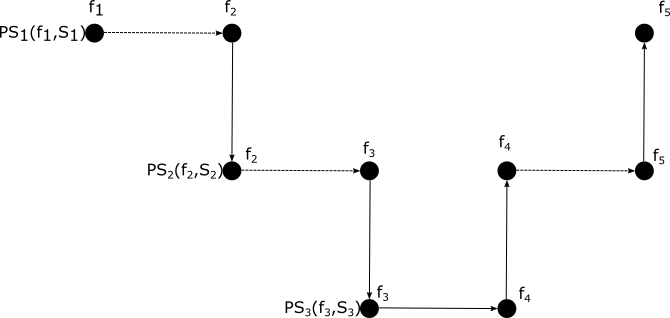
\includegraphics[width=\linewidth]{mc.png}
	\caption{Model Checking Procedure.}
	\label{fig:mc}
\end{figure}

Can also be adjusted for \textbf{recursive} method calls:

\begin{itemize}
	\item Need to register "partial" proof structures in registry/ interprocedural analysis in order to map proof structures to method calls	
	\item Model checking happens offline, not on-the-fly since state spaces could not be reused for recomputation
\end{itemize}

On-the-fly model checking is basically based on the new method generateAndCheck() in StateSpaceGenerator class. Methods that use generate():

\begin{todolist}
	\item CounterExampleGenerator
	\item[\done] InterproceduralAnalysis.run()
	\item[\done] InternalPartialStateSpace.continueExecution()
	\item[\done] InternalProcedureCall.execute()
	\item InternalContractGenerator
	\item AbstractMarkingGenerator
\end{todolist}

\subsubsection{To-Do}
\begin{todolist}
	% \item[\done] for ticked boxes \item[\wontfix] for crossed boxes
	
	\item[\done] Set abort criteria	
	\item[\done] Example: refSll should visit \textbf{all} states
	\item[\done] Example: MC\_completeness\_reverseWithInitialList has no final states: \textit{Model checking terminates before reaching final states, thus they do not need to be generated}
	\item[\done] Generate recursive example
	\item[\done] Send back formulae resulting from model checking to upper state spaces 
	\item[\done] Contract generation
	\begin{itemize}
		\item when are contracts used? 
		\item failed Model Checking: abort, no contracts necessary
		\item successful Model Checking: complete state space needed, but maybe not generated if declared successful early (e.g. for Xf)
		\item \textbf{ Generate complete state space if model checking was successful} and not complete state space generated yet: 
		\begin{itemize}
			\item mark states as explored in stateSpaceGenerator 
			\item continue generation with unexplored states --> generate() 
			\item generate post and preconditions
		\end{itemize} 
		\item return true when sub-proof structure is successful
		\item how to handle false proof structures? 
	\end{itemize}
	\item[\done] Store model checking results to avoid multiple checks of the same state space/ method $\rightarrow$ store results
	\item[\done] Adjust contract matching method to consider different input formulae for model checking
	\item Abort model checking as soon as a failure is found in a procedure state space (use boolean variable buildFullStructure to also allow for full model checking)	
	\item Refactor state space generator
	\item Debug time issue of hierarchical model checking
	\item Reuse partial graphs for model checking (generate new states if needed) - map proof structure to the same (continuing) state space
	\item totalStatesCounter is at wrong position in generateAndCheck() method.. should only be called once for each state space	
	\item Generate more examples for testing procedure model checking 
\end{todolist}

\subsubsection{Notes}

\begin{itemize}
	\item Procedure call examples: G \{L(SLL)\} fails if method with list object is called by another method, e.g. main because the main state space is not a list
	\item Constructor calls fail procedure model checking because they are started with initial empty heap; need to exclude them from procedure model checking and only use contracts on current heap
\end{itemize}

\subsection{Hierarchical Model Checking (offline)}
(2 weeks)\\

\textbf{Possible approach:}
\begin{itemize}
	\item Create RSM from procedure state spaces
	\item Model check state spaces separately
	\item Get global failure trace
\end{itemize}

\subsubsection{To-Do}
\begin{todolist}
	\item[\done] Implement recursive model checking in offline manner, but with hierarchical use of results: generate RSM out of procedure state spaces	
\end{todolist}

\subsection{Global To-Do's}
\begin{todolist}
	\item Implement mechanism to decide on which procedures are checked and which not
	\item Run Java Tests for proof structure
		\begin{todolist}
			\item[\done] TableauRulesSwitch2
			\item[\done] ProofStructure2 (SimpleProofStructure)
			\item HierarchicalProofStructure
			\item OntheflyProofStructure
			\item ModelCheckingContracts
			\item Mechanism to decide which procedures to check
			\item RSM
		\end{todolist}
	\item Generate output report (diagram)
	\item Add statistics to model checking summary
	\item Clean up code
	\item Write down implication relations for LTL formula (use for model checking contracts)
	\item Compare offline and on-the-fly model checking
\end{todolist}

\subsection{Extensions}	
\subsubsection{Statically imply model checking results from LTL-formulae}
\subsubsection{Pre-Model Checking of procedures/ contracts}
(2 weeks)
After procedure state space has been completely generated, model check state space for all sub-formulae of the initial LTL formula  $\varphi$: $\mathcal{O}(3^n)$ sub-formulae where $n$ is the number of sub-formulae in $\varphi$.	

\subsubsection{Program generation from counterexample trace}
(2 weeks)

\end{document}
